%%%%%%%%%%%%%%%%%%%%%%%%%%%%%%%%%%%%%%%%%%%%%%%%%%%%%%%%%%%%%%%%%%%%%%%%%%%%%%%%%%%%%%
% TEMPLATE FOR Praktikum P3B
% This template uses the Memoir class. It is a very powerful class for creating documents such
% as reports, papers and theses. You can find more information at CTAN, the Comprehensive
% TeX Archive Network. These is a long manual that describes how to use Memoir.
% https://www.ctan.org/pkg/memoir?lang=en
% Sven Buschke
% Last Update: 2021-08-18
%%%%%%%%%%%%%%%%%%%%%%%%%%%%%%%%%%%%%%%%%%%%%%%%%%%%%%%%%%%%%%%%%%%%%%%%%%%%%%%%%%%%%

%------------------------------------------------------------------------------------
%	EDIT THIS BLOCK
%------------------------------------------------------------------------------------
\newcommand{\studentfullname}{Sven Buschke}			% change to your name
\newcommand{\matrikelnumber}{27205317}				% enter your student number 
\newcommand{\dateexperiment}{20. August 2021}				% change to your partner's name
\newcommand{\timeexperiment}{13:45-18:15 Uhr}				% enter your partner's student number
\title{P3B-Versuch 4C SPL --- Spektrallinien}					% change to the title of the experiment
\author{\studenfullname}				% you don't have to change this
\date{23.\ August 2021}										% this fills in today's date - don't change



%------------------------------------------------------------------------------------
%	FORMATTING STUFF
%------------------------------------------------------------------------------------

\documentclass[12pt,oneside,oldfontcommands]{memoir}


%-----------------------------------------------------------------------------------
%	MARGIN AND HEADER/FOOTER SIZES
%------------------------------------------------------------------------------------
\setlrmarginsandblock{2.5cm}{2.5cm}{*}  		% left/right margins
\setulmarginsandblock{2.5cm}{2.5cm}{*} 			% top/bottom margins
\checkandfixthelayout							% checks the layout is correct
\setlength{\parindent}{0in}  					% no indent on start of paragraph
							

%-------------------------------------------------------------------------------------
%  PACKAGES
%-------------------------------------------------------------------------------------
\usepackage{amsmath,amsthm,amssymb,amsfonts}			% math fonts
\usepackage[german]{babel}								% hyphenation rules for German
\usepackage{graphicx}									% for importing pdf files 
\usepackage{siunitx}									% si units - extremely useful
\usepackage[usenames,dvipsnames,svgnames,table]{xcolor}	% defines the dvips color names
\usepackage{color,soul} 								% for highlight hi - hyphenation, underlining
%\usepackage{libertine}
%\usepackage{libertinust1math}
%\usepackage[T1]{fontenc}
\usepackage{fontspec}
\usepackage{pdfpages}
\setmainfont{Linux Libertine O}%
   [Ligatures={Common,Rare,Historic}, Numbers=OldStyle]
\setulcolor{red} 										% set underline color
\setstcolor{green} 										% set overstriking color
\sethlcolor{green} 										% set highlighting color


%--------------------------------------------------------------------------------------------
%  GRAPHICS PATH
%--------------------------------------------------------------------------------------------
\graphicspath{{figures/}}								% put your figures in a folder called figures



%---------------------------------------------------------------------------
%  SOME NEW FUNCTIONS FOR IMPORTING FIGURES
%---------------------------------------------------------------------------
\newcommand{\placefigure}[1]{\centerline{\includegraphics[width=2 in]{#1}}} 
\newcommand{\placefigureandscale}[2]{\centerline{\includegraphics[width=#2 in]{#1}}} 



%-------------------------------------------------------------------------------------
%	TITLE PAGE MACRO
%------------------------------------------------------------------------------------
\makeatletter
\def\maketitle{%
  \null
  \thispagestyle{empty}
  \begin{center}\leavevmode
       \normalfont 	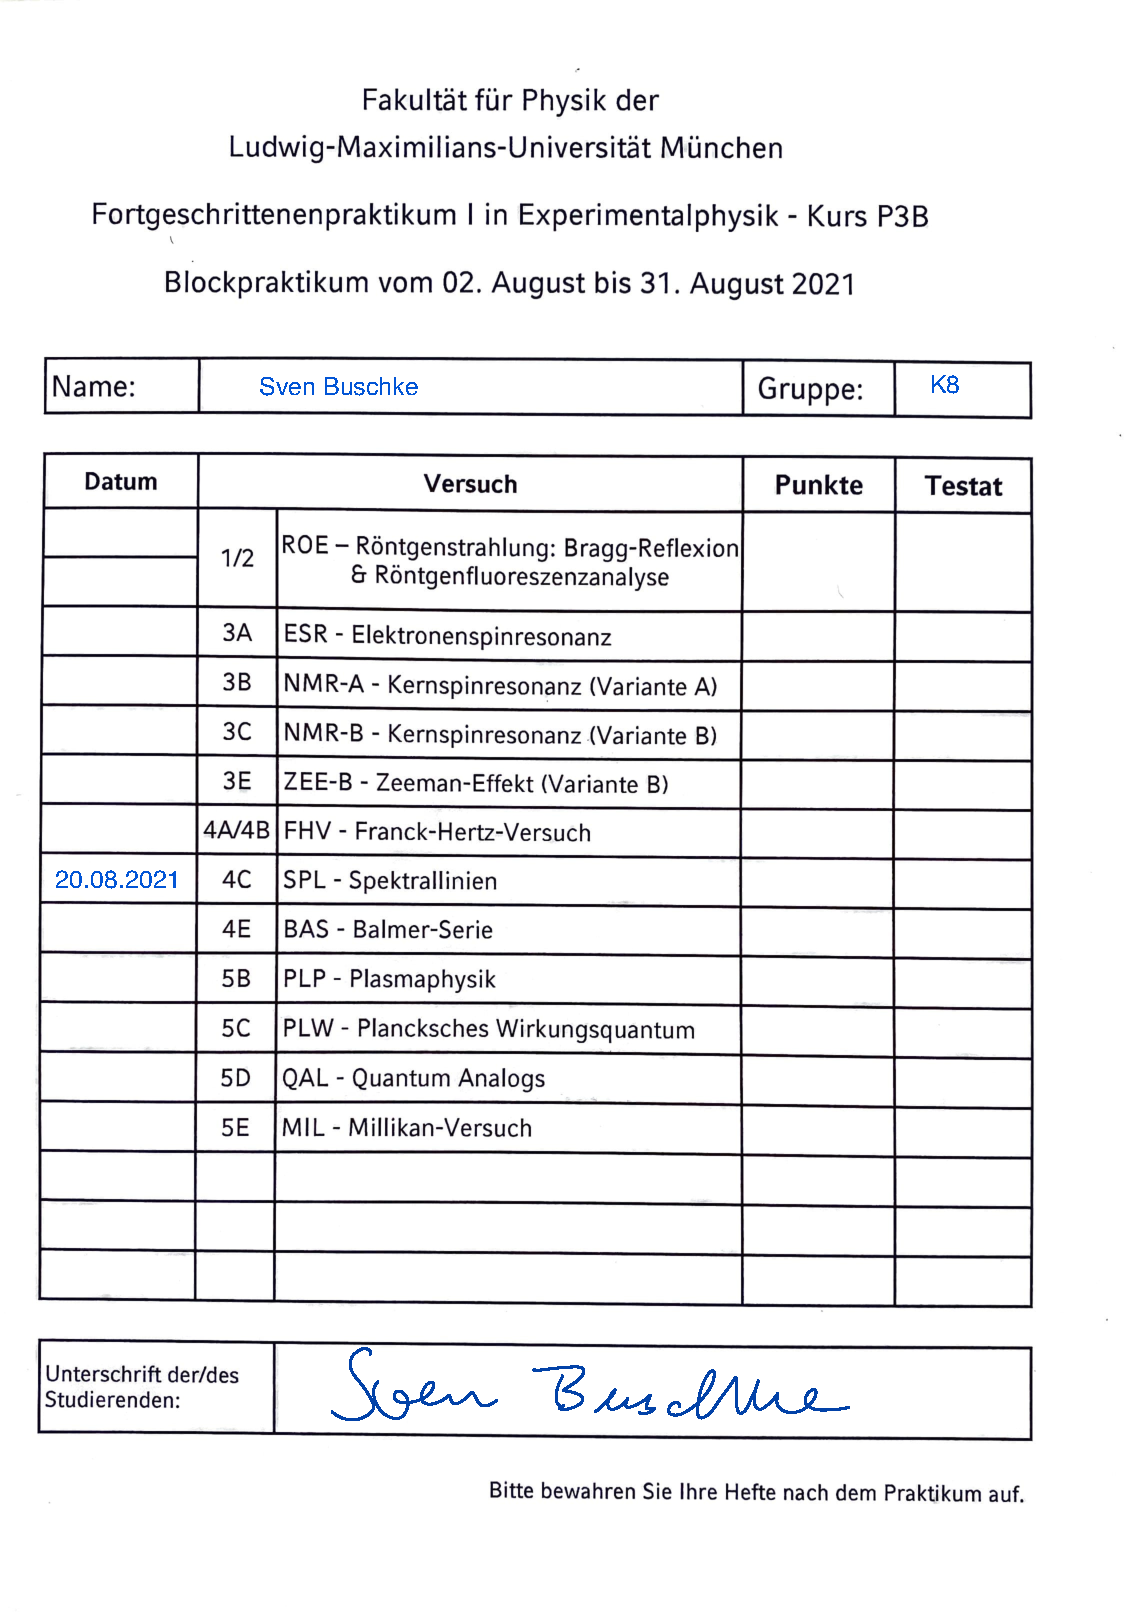
\includegraphics[width=.96\columnwidth]{Deckblatt-P3B-signed-20210820-sb.pdf}
       \newpage
       
\includegraphics[width=0.165\columnwidth]{lmu-seal.pdf}
       
\includegraphics[width=0.35\columnwidth]{lmu-logo.pdf}
       \vskip 0.5cm   
       \textsc{\Large P3B-Praktikum}\\[0.5 cm]
	     {\large \@date\par}
       \vskip 1.0cm
	\rule{\linewidth}{0.2 mm} \\[0.4 cm]
	{ \huge \bfseries \@title}\\
	\rule{\linewidth}{0.2 mm} \\[1.5 cm]
	
	\begin{minipage}{0.5\textwidth}
		\begin{flushleft} \large
			\emph{Name:} \studentfullname\\
			Matrikelnummer: \matrikelnumber
			\end{flushleft}
			\end{minipage}~
			\begin{minipage}{0.4\textwidth}
			\begin{flushleft} \large
			Versuchstermin: \dateexperiment\\
			Versuchsdauer: \timeexperiment
		\end{flushleft}
	\end{minipage}\\[2 cm]
   \end{center}
   \vfill
   \null
   \cleardoublepage
  }
\makeatother



%-------------------------------------------------------------------------------------------
%	START OF DOCUMENT
%--------------------------------------------------------------------------------------------

\begin{document}
%\large 
\maketitle
\frontmatter
\let\cleardoublepage\clearpage
\mainmatter
\sloppy



%--------------------------------------------------------------------------------------------
%	RESULTS AND ANALYSIS
%--------------------------------------------------------------------------------------------

\setcounter{tocdepth}{3}
\tableofcontents

\section{Vorbereitung Versuch 4C SPL}
\subsection{Physikalische Grundlagen}
Mit diesem Versuch sollen sichtbare Spektrallinien unterschiedlicher Elemente bestimmt werden.
\subsubsection{Stichworte}
\paragraph{Hamilton-Operator des Wasserstoffs}

\paragraph{Hamilton-Operator für Mehrteilchensysteme}
\paragraph{Termschema der Elektronen}
\paragraph{Schrödinger-Gleichung}
\paragraph{Wellenansatz zur Lösung der Schrödinger Gleichung}
\paragraph{Quantenzahlen eines Atoms}
\paragraph{Drehimpulsoperator $\vec{L}$}


Photoemission\\
Plancksches Wirkungsquantum $h = 6.6261 \cdot 10^{34} Js$ \\
Es gilt $hv=E_1-E_0$\\

Schrödinger Gleichung $\hbar = h/2\pi$\\

Herleitung
$i \hbar \frac{\partial}{\partial t} \psi(\vec{r},t) = H \psi(\vec{r},t)$

Eigenfunktion des Hamiltonoperators

$\hat{H} = \frac{-\hbar^2}{2m} \nabla^2 + V(\vec{r},t)\\$

Wellenfunktion
$\psi(\vec{r},t) = A exp(i(\vec{k}\vec{r} - \omega t))$ \\
zeitunabhnägige Schrödinger-Gleichung: $\hat{H} \psi (\vec{r}) = E \psi(\vec{r})$

Wasserstoff-Atom, zeitunabhängige Schrödinger-Gleichung:  %$\frac{\hbar^2}{2m_e}(\frac{\partial^2}{\partial r^2}+\frac{2}{r}\frac{\partial}{\partial r}))+ \frac{\vec{L}^2}{2m_er^2}+V(\rec{r}] \psi(\vec{r} = E \psi(\vec{r})$

Coulombpotenzial H-Atom: $V(r) = -Z e^2 / (4 \pi \epsilon_0 r)$\\

Separationsansatz: $\psi(\vec(r) = \frac{R(r)}{r}Y_{lm_l}(\theta, \phi)$\\

Potenzreihenansatz: $P(r) \sum^\infty_{\mu = 0} = \alpha_{\mu}$

Energieniveaus: $E_n = -\frac{Z^2 E_R}{n^2} = - \frac{m_e Z^2 e^4}{8 \epsilon^2_0 h^2} \cdot {1}{n^2}$ \\

Rydbergenergie: $E_R = hcR_{\infty}$

allgmeines Seriengesetz: $v = \frac{c}{\lambda} = \frac{E_m - E_n}{h} = \frac{m_e e^4}{8 \epsilon_0^2 h^3} [\frac{1}{n^2} - \frac{1}{m^2}] \Longleftrightarrow \frac{1}{\lambda} = R_\infty [\frac{1}{n^2} - \frac{1}{m^2}]$\\

Rydbergenergie: $E_R = hcR\infty$\\

Teilversuch 2:

Hamilton Operator:

$H = \frac{p^2_1}{2m_e} - \frac{1}{4\pi \epsilon_0} $

$H = H_1 + H_2 + H_{WW}$ \\

Wechselwirktungsterm $H_{WW} = $ \\

Wechselwirkungsterm als Störung des Hamiltonoperators $H'$\\


Eigenfunktionen $| \Psi >$\\

Eigenwerte 1. Ordnung von H: $E = E^0_n = \Delta E_{WW}$\\

$\Delta_{WW} = < \Psi | H_{WW} | \Psi >$\\

Teilversuch 3:\\

Notation der Übergänge:\\
übliche Notation der Spektroskopie: L Bahndrehimpuls L, S für L = 0]\\


Auswahlregeln:\\
Aufnahme passendes Lichtquants, Absorption Spektrallinie\\
Abgabe eines Quants\\

Bahndrehimpulsqunatenzahl L ändert sich um 1 (Dipolcharatker des Übergangs)\\

Angeregte Atome in einer Spektrallampe\\

Thermische Ionisation\\

Elektronenstoßionisation\\

Photoionisation\\

Glimmentladung\\

Bogenentladung\\

Bestimmung der Wellenlängen der emittierten Photonen\\

Beugung am Gitter\\

Grotrian-Diagramme\\



Teilversuch 4:\\


\subsubsection{Theoretischer Hintergrund}
\paragraph{Teilversuch 1: Das Einelektronensystem}
\paragraph{Teilversuch 2: Helium-Spektrum (Zweielektronensystem mit leichtem Atomkern)}
\paragraph{Teilversuch 3: Quecksilber-Spektrum (Mehrelektronensystem mit schwerem
Kern)}
\paragraph{Teilversuch 4: Demonstration der Aufspaltung von Spektrallinien}
\paragraph{Teilversuch 5: Qualitative Analyse der Spektren anderer Atome bzw.
Moleküle}
\paragraph{Teilversuch 6: Qualitative Analyse des Spektrums der Spektralröhre mit Luft
}

\section{Versuchsdurchführung und Auswertung}
\subsection{Teilversuch 1: Das Einelektronensystem}
\subsubsection{Versuchsvorbereitung}
\paragraph{Grundlagen des Versuchs}
In diesem Teilversuch sollen gemäß Versuchsanleitung ...:
%\begin{enumerate}
%    \item eins
%    \item 
%\end{enumerate}

\paragraph{Erläuterung verwendeter Formelzeichen}
\paragraph{Versuchsziel}



\paragraph{Erläuterung der Messmethoden}
\paragraph{schematische Skizzen}
Versuchsaufbau\\

Spektralröhrenneztgerät\\
Spektrallampe\\

Gitte im Abstand von 45 cm zur Skala aufstellen\\

Wasserstoffspektralröhre zu verwenden\\

Spannung von 5 kV notwendig \\

Gitte möglichst parallel zur Skala auszurichten\\

Bestimmung Abstand d des Gitters von der Skala\\

im abgedunkelten Raum leuchtende Kapillare der Spektralröhre durch das Gitter zu betrachten\\

Ohne Kopfbewegung nun Abstand 2l messen\\

Berechnen aus den Messwerten die Wellenlängen und ordnen die Übergänge zwischen den Elektronniveaus in spektroskopischer Darstellung zu\\

Ermitteln des experimentellen Wertes für die Rydbergkonstante und Abschätzung des Fehlers. Geeignete Abschätzungsmethode:\\


\paragraph{Planung der Durchführung}
\subsubsection{Versuchsplanung}
\subsubsection{Versuchsdurchführung}
\subsubsection{Versuchsergebnisse und -auswertung}
Rot: links: 31,9 cm\\
rechts: 64,55 cm\\

Fehlerabschätzung: plus minus 0,05 cm\\




\subsection{Teilversuch 2: Helium-Spektrum (Zweielektronensystem mit leichtem Atomkern)}
\paragraph{Erläuterung verwendeter Formelzeichen}
\paragraph{Versuchsziel}
\paragraph{Erläuterung der Messmethoden}
\paragraph{schematische Skizzen}

Heliumspektralröhre, daher Ersetzen Wasserstoffspektralröhre durch Helumröhre\\

Messen der Abstände 2l und d, Berechnen der Wellenlängen der beobachteten Spektrallinien\\

Ordnen der Wellenlängen zu den zugehörigen Elektronenübergänge im Grotrian-Diagramm\\

Tabelle mit den Übergängen in spektroskopischer Notation aus Termschema\\



\paragraph{Planung der Durchführung}
\subsubsection{Versuchsplanung}
\subsubsection{Versuchsdurchführung}
\subsubsection{Versuchsergebnisse}
\subsubsection{Versuchsauswertung}

\subsection{Teilversuch 3: Quecksilber-Spektrum (Mehrelektronensystem mit schwerem
Kern)}
\paragraph{Erläuterung verwendeter Formelzeichen}
\paragraph{Versuchsziel}
\paragraph{Erläuterung der Messmethoden}
\paragraph{schematische Skizzen}

Analoge Messung zu Teilversuch 2 mit Quecksilberröhre\\

Mögliche Aufspaltung einzelner Spektrallinien\\

Messen Abstände 2l und d\\

Betrachten der Wellenlängen der Spektrallinien\\

Anordnung der Elektronenübergänge im Grotrian Diagramm\\

\paragraph{Planung der Durchführung}
\subsubsection{Versuchsplanung}
\subsubsection{Versuchsdurchführung}
\subsubsection{Versuchsergebnisse}
\subsubsection{Versuchsauswertung}

\subsection{Teilversuch 4: Demonstration der Aufspaltung von Spektrallinien}
\paragraph{Erläuterung verwendeter Formelzeichen}
\paragraph{Versuchsziel}
\paragraph{Erläuterung der Messmethoden}
\paragraph{schematische Skizzen}

Aufbau Spektrogoniometers und SPektrallampe, ohne Messchieber\\

Beobachten der Spektrallinien verschiedner Elemente, (Hg und Na) mit Spektrogoniometer\\

Beschreiben und Begründung der Beobachtungen\\

\paragraph{Planung der Durchführung}
\subsubsection{Versuchsplanung}
\subsubsection{Versuchsdurchführung}
\subsubsection{Versuchsergebnisse}
\subsubsection{Versuchsauswertung}

\subsection{Teilversuch 5: Qualitative Analyse der Spektren anderer Atome bzw.
Moleküle}
\paragraph{Erläuterung verwendeter Formelzeichen}
\paragraph{Versuchsziel}
\paragraph{Erläuterung der Messmethoden}
\paragraph{schematische Skizzen}

Aufbau von Teilversuch 1\\

Betrachtung der Spetren von $N_2$, $O_2$, $H_2O$ und $A_r$\\

Beschreibung des Unterschieds zwischen den Spektren von Atomen und Molekülen\\

Erklärung der Ursachen für den Unterschied.\\

\paragraph{Planung der Durchführung}
\subsubsection{Versuchsplanung}
\subsubsection{Versuchsdurchführung}
\subsubsection{Versuchsergebnisse}
\subsubsection{Versuchsauswertung}

\subsection{Teilversuch 6: Qualitative Analyse des Spektrums der Spektralröhre mit Luft}
\paragraph{Erläuterung verwendeter Formelzeichen}
\paragraph{Versuchsziel}
\paragraph{Erläuterung der Messmethoden}
\paragraph{schematische Skizzen}

Aufbau von Teilversuch 1\\

Betrachtung des Spektrum der Spektralröhre mit Luft\\

Welche Bestandteile in Luft müssen enthalten sein\\

Auswahl entsprechnder Spektralröhre\\

Überprüfung der Vermutungungen durch Vergleich mit Spektren bei nur einer Atom- und Molekülsorte.\\

\paragraph{Planung der Durchführung}
\subsubsection{Versuchsplanung}
\subsubsection{Versuchsdurchführung}
\subsubsection{Versuchsergebnisse und Versuchsauswertung}

\section{Anhang - Fotos}
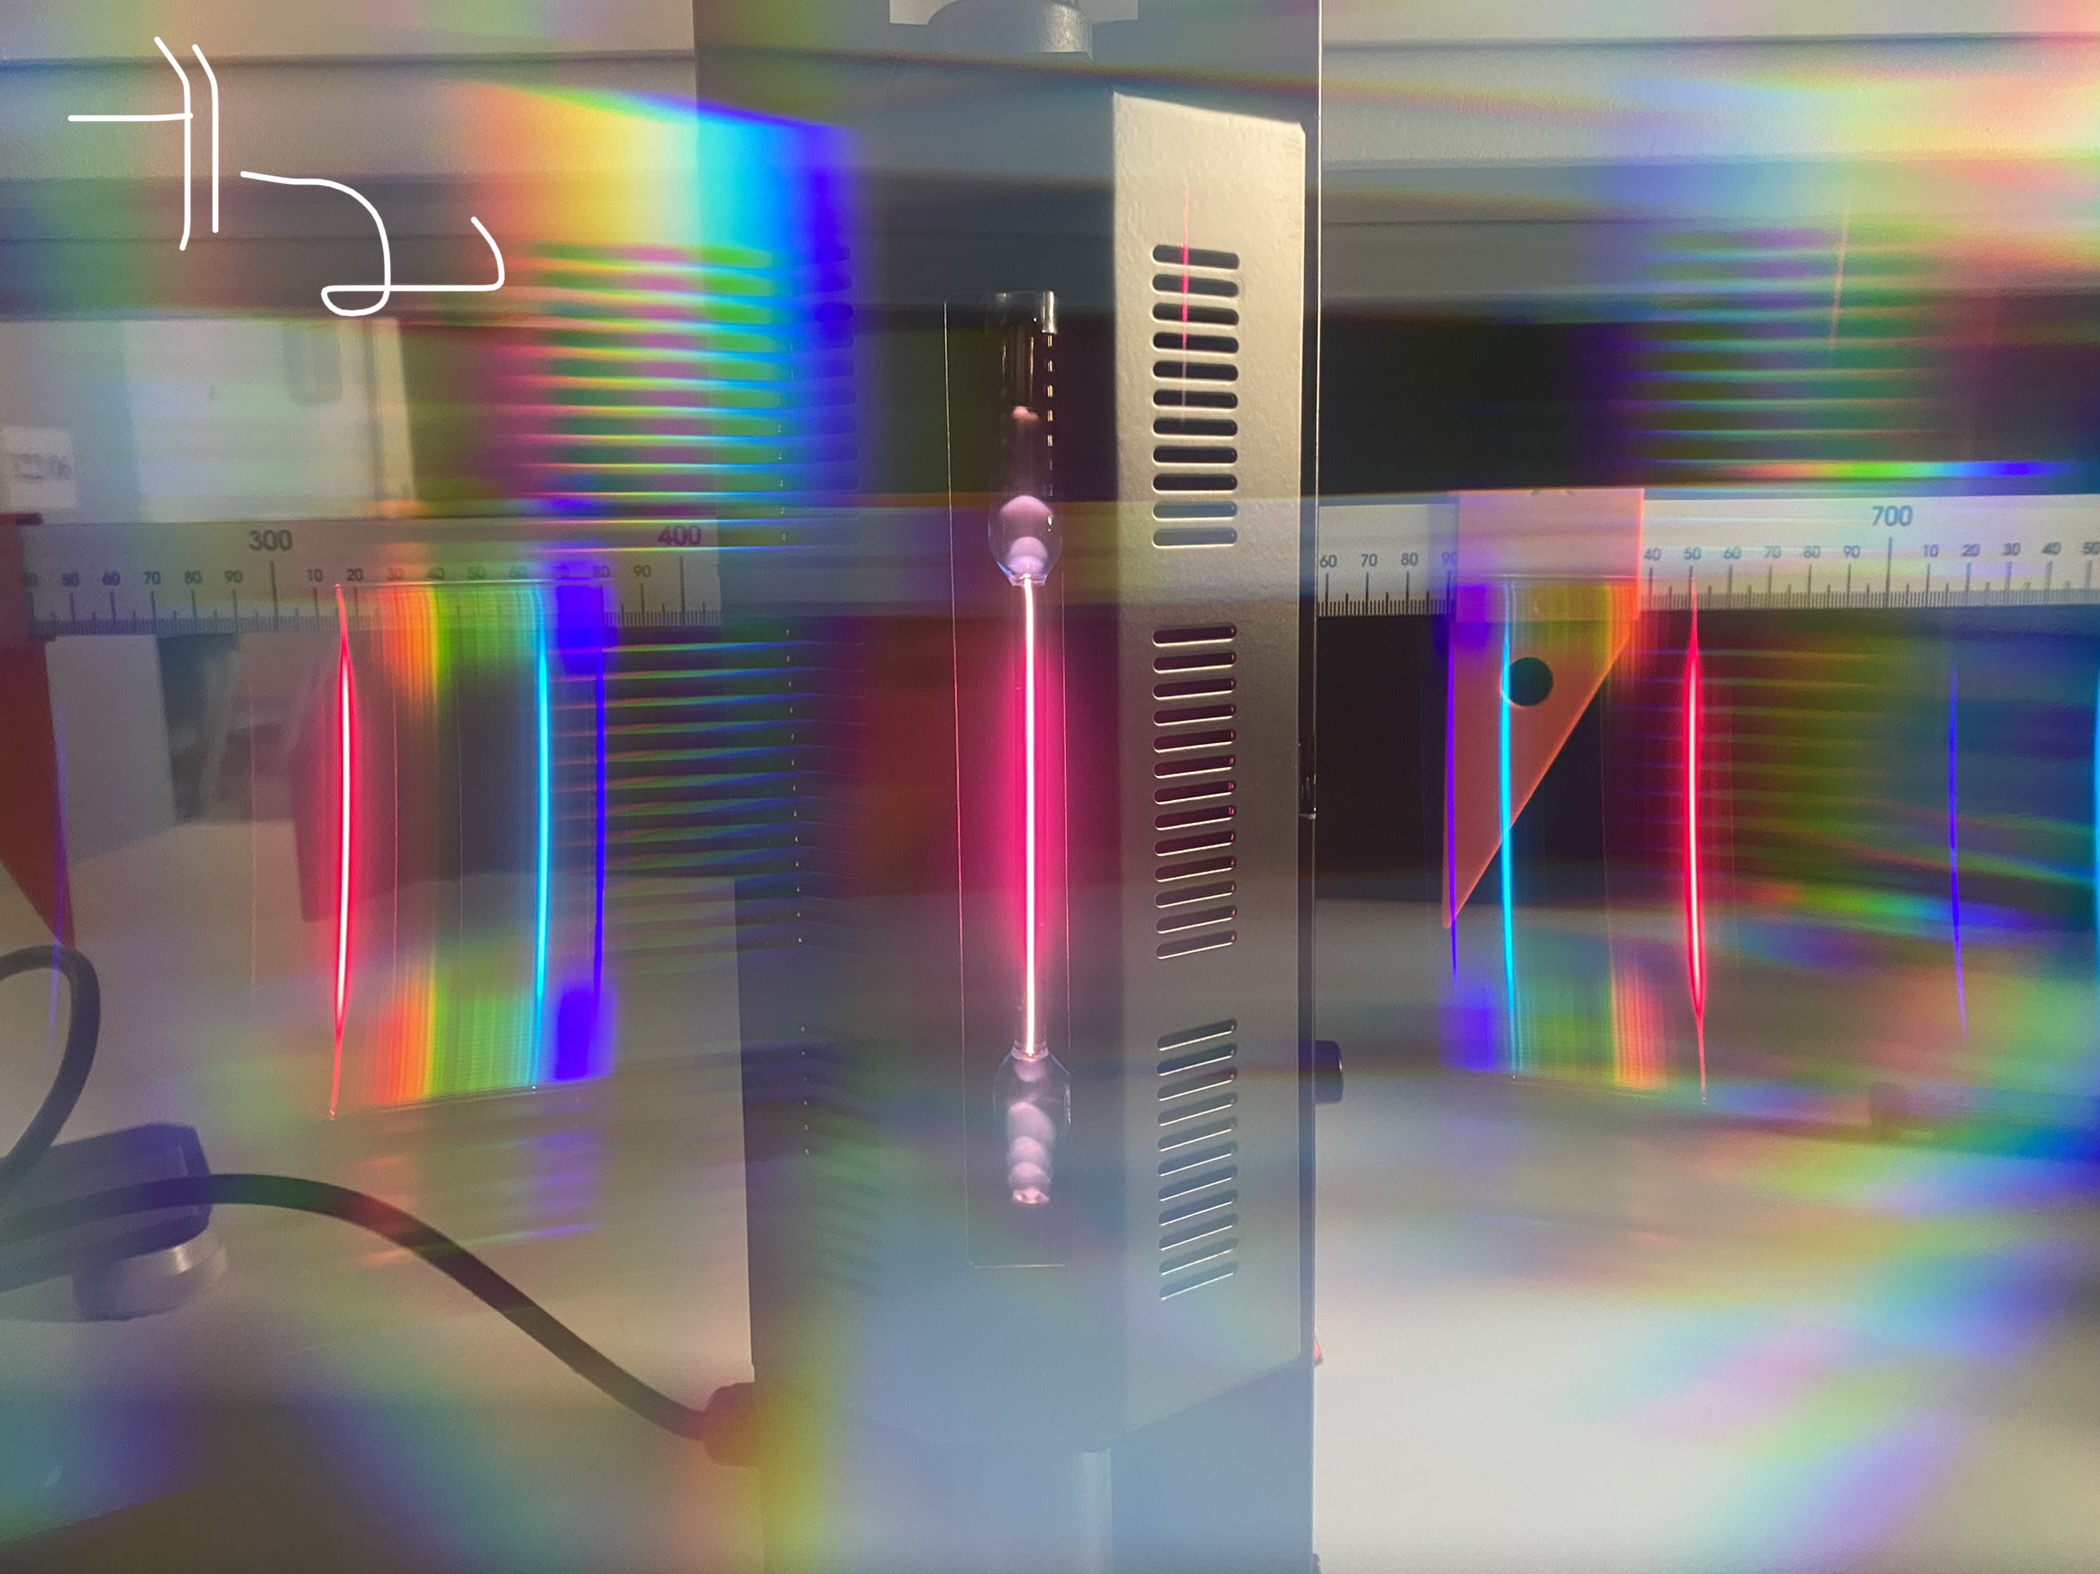
\includegraphics[width=.96\columnwidth]{figures/IMG_5291.jpg}
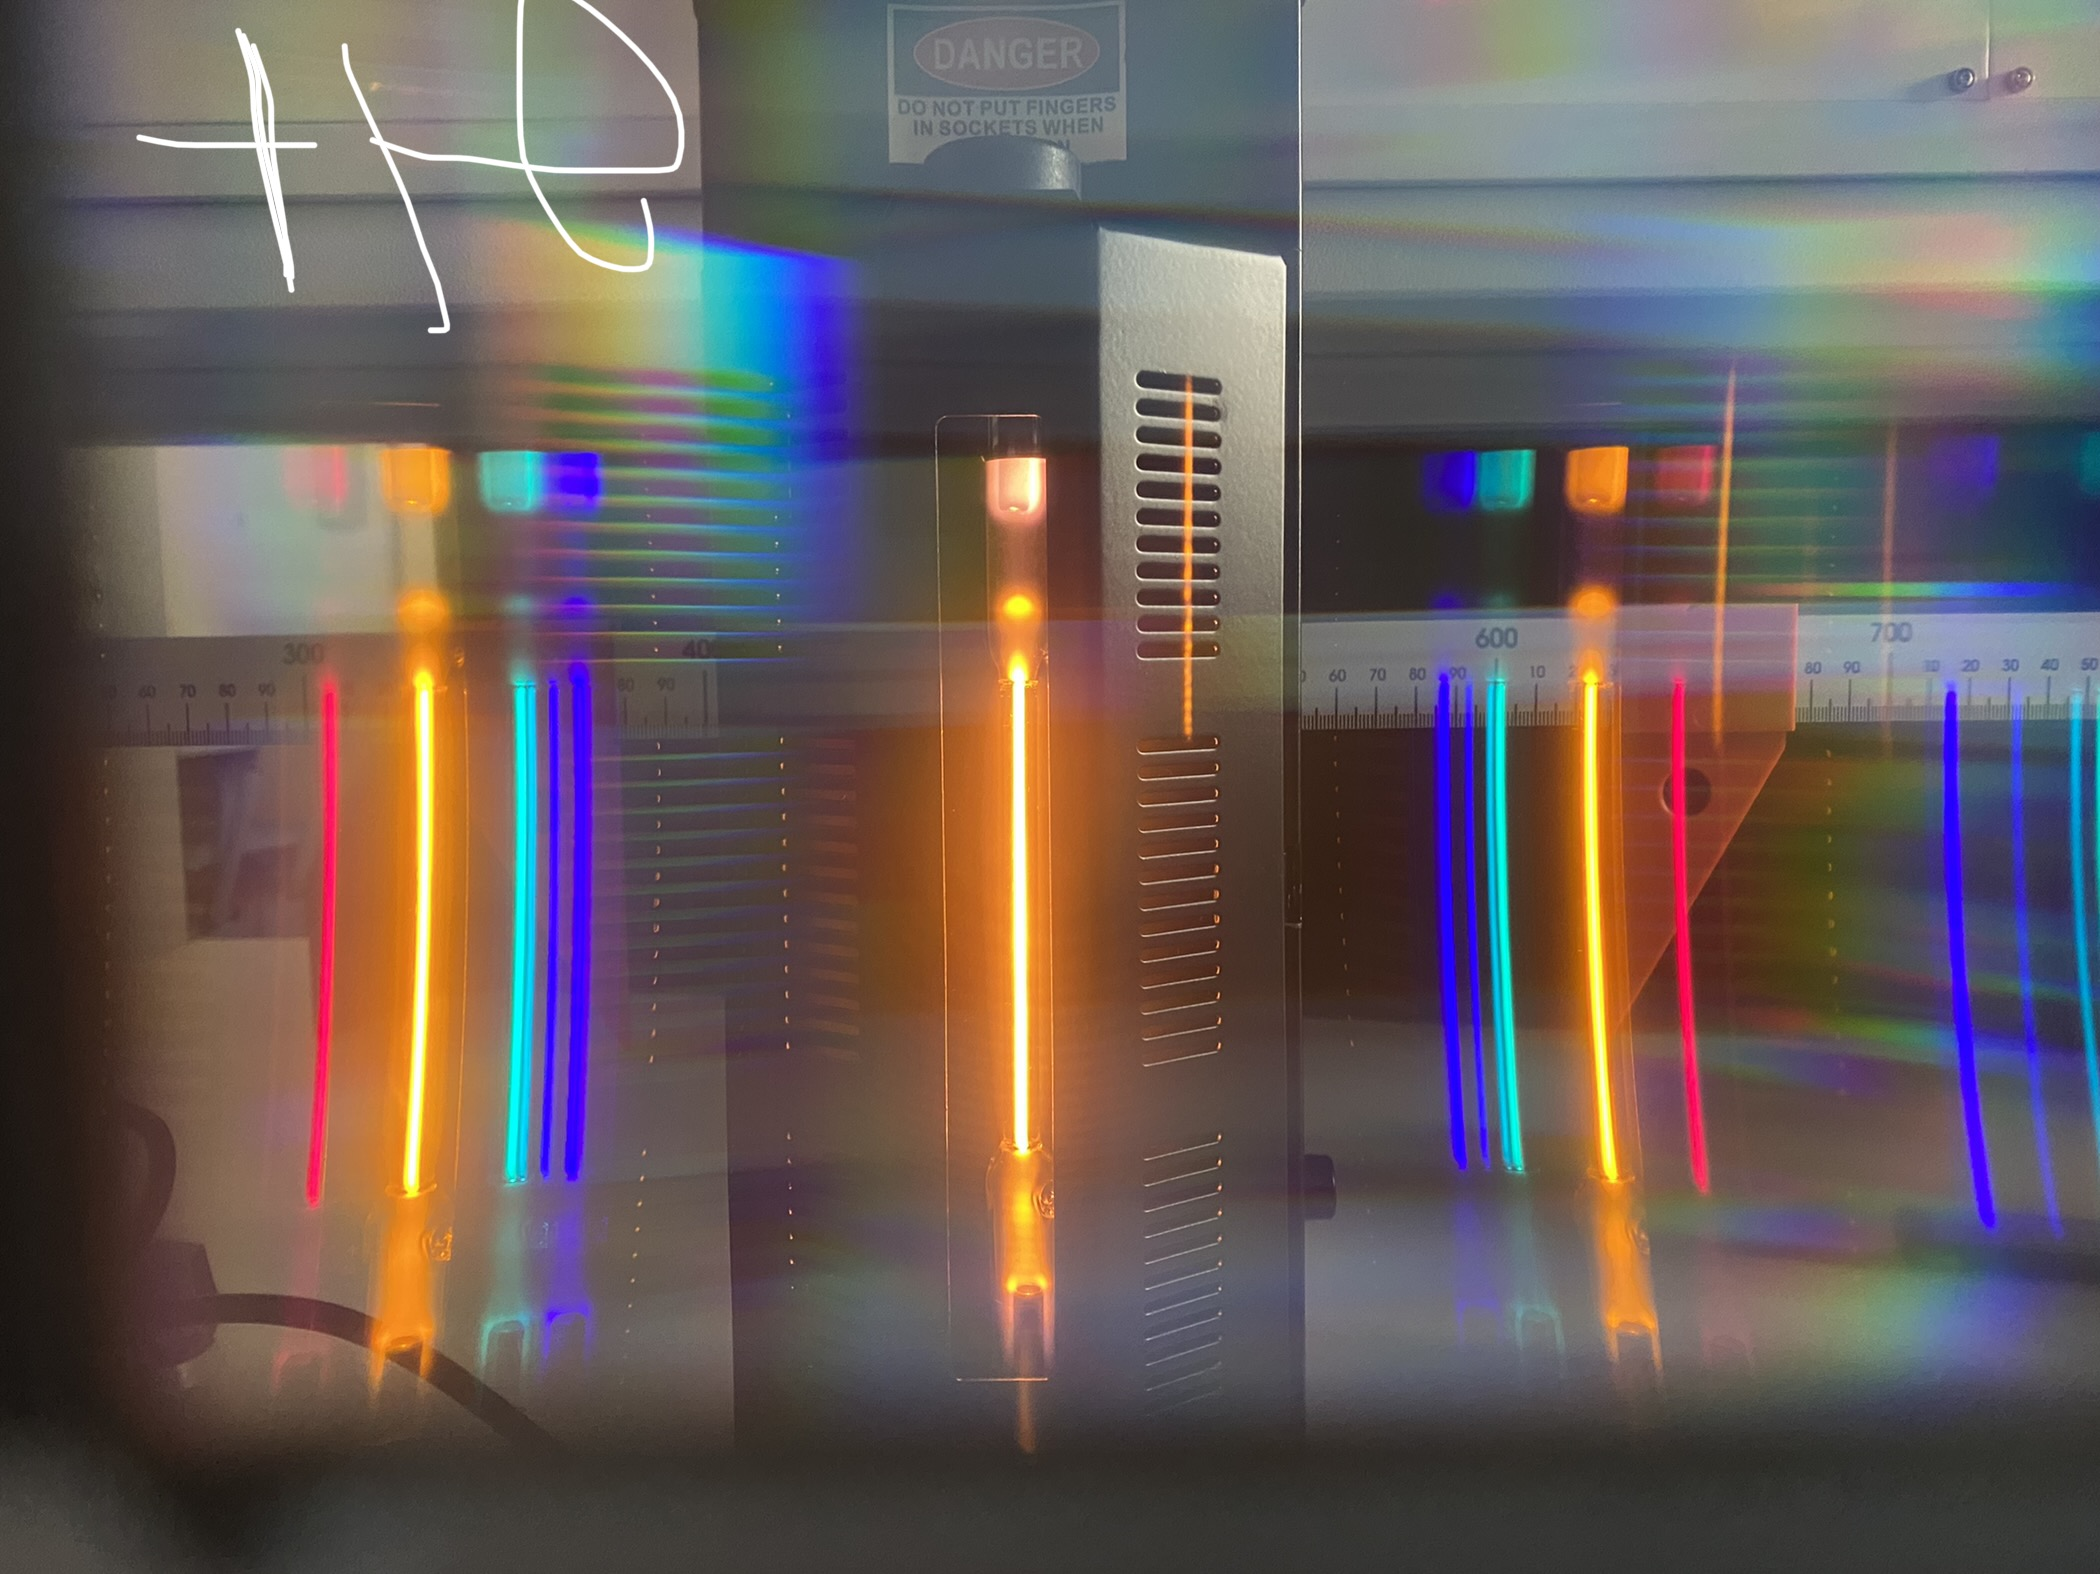
\includegraphics[width=.96\columnwidth]{figures/IMG_5292.jpg}
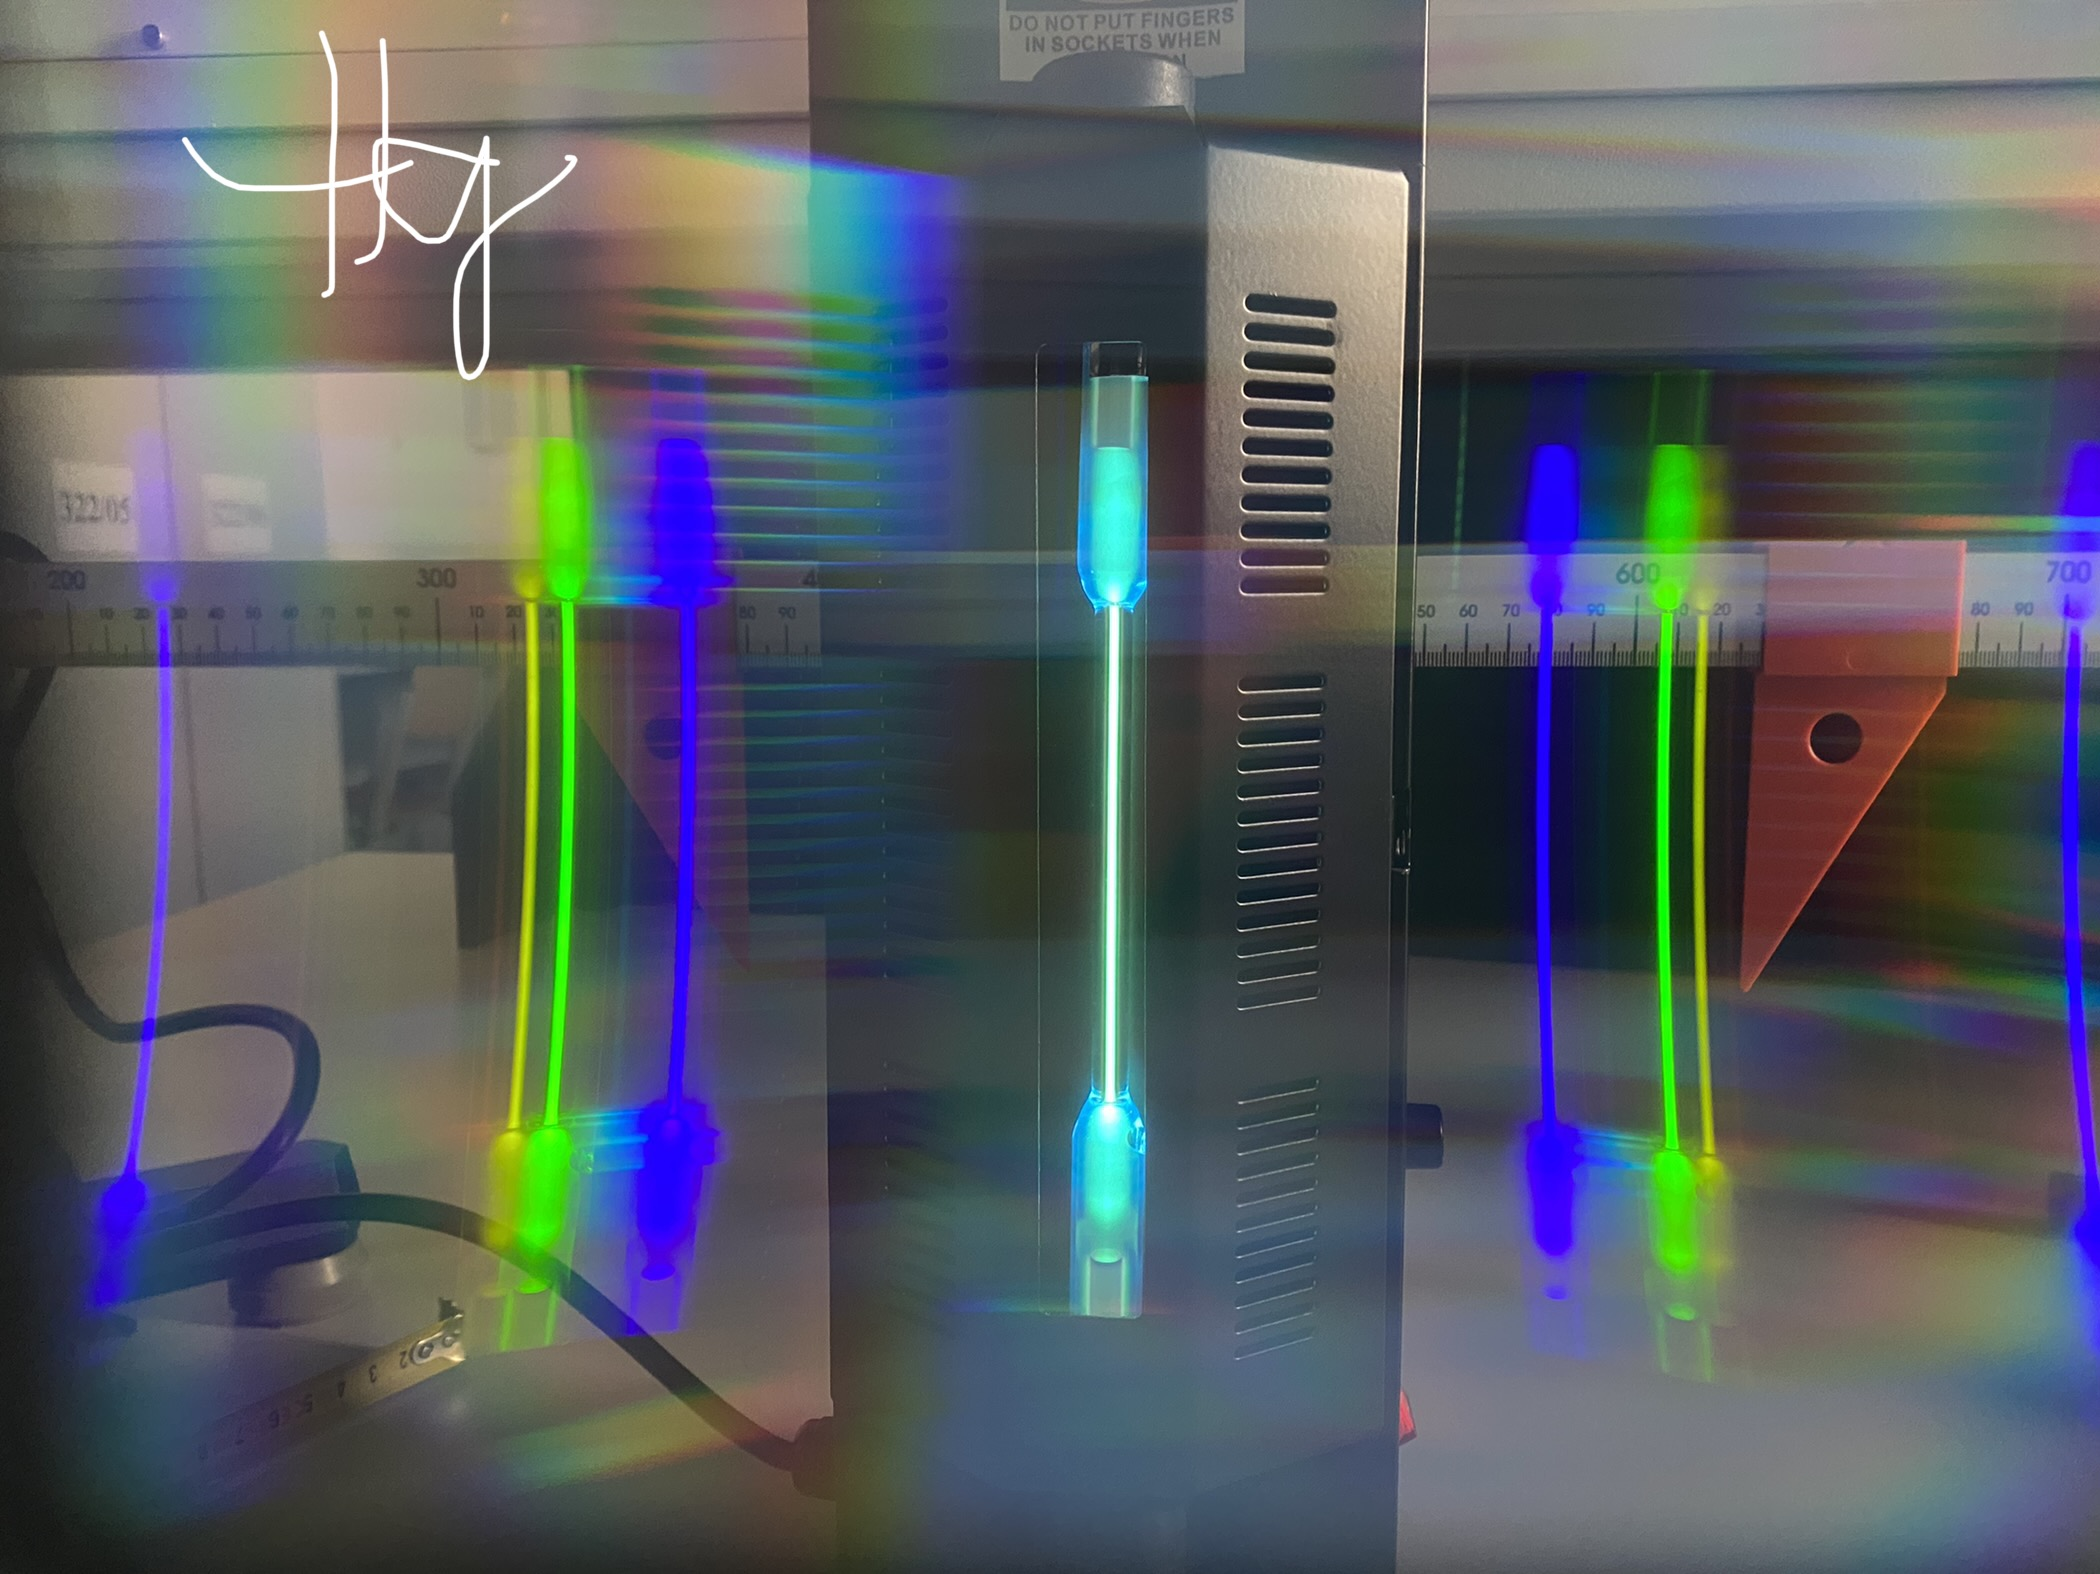
\includegraphics[width=.96\columnwidth]{figures/IMG_5293.jpg}
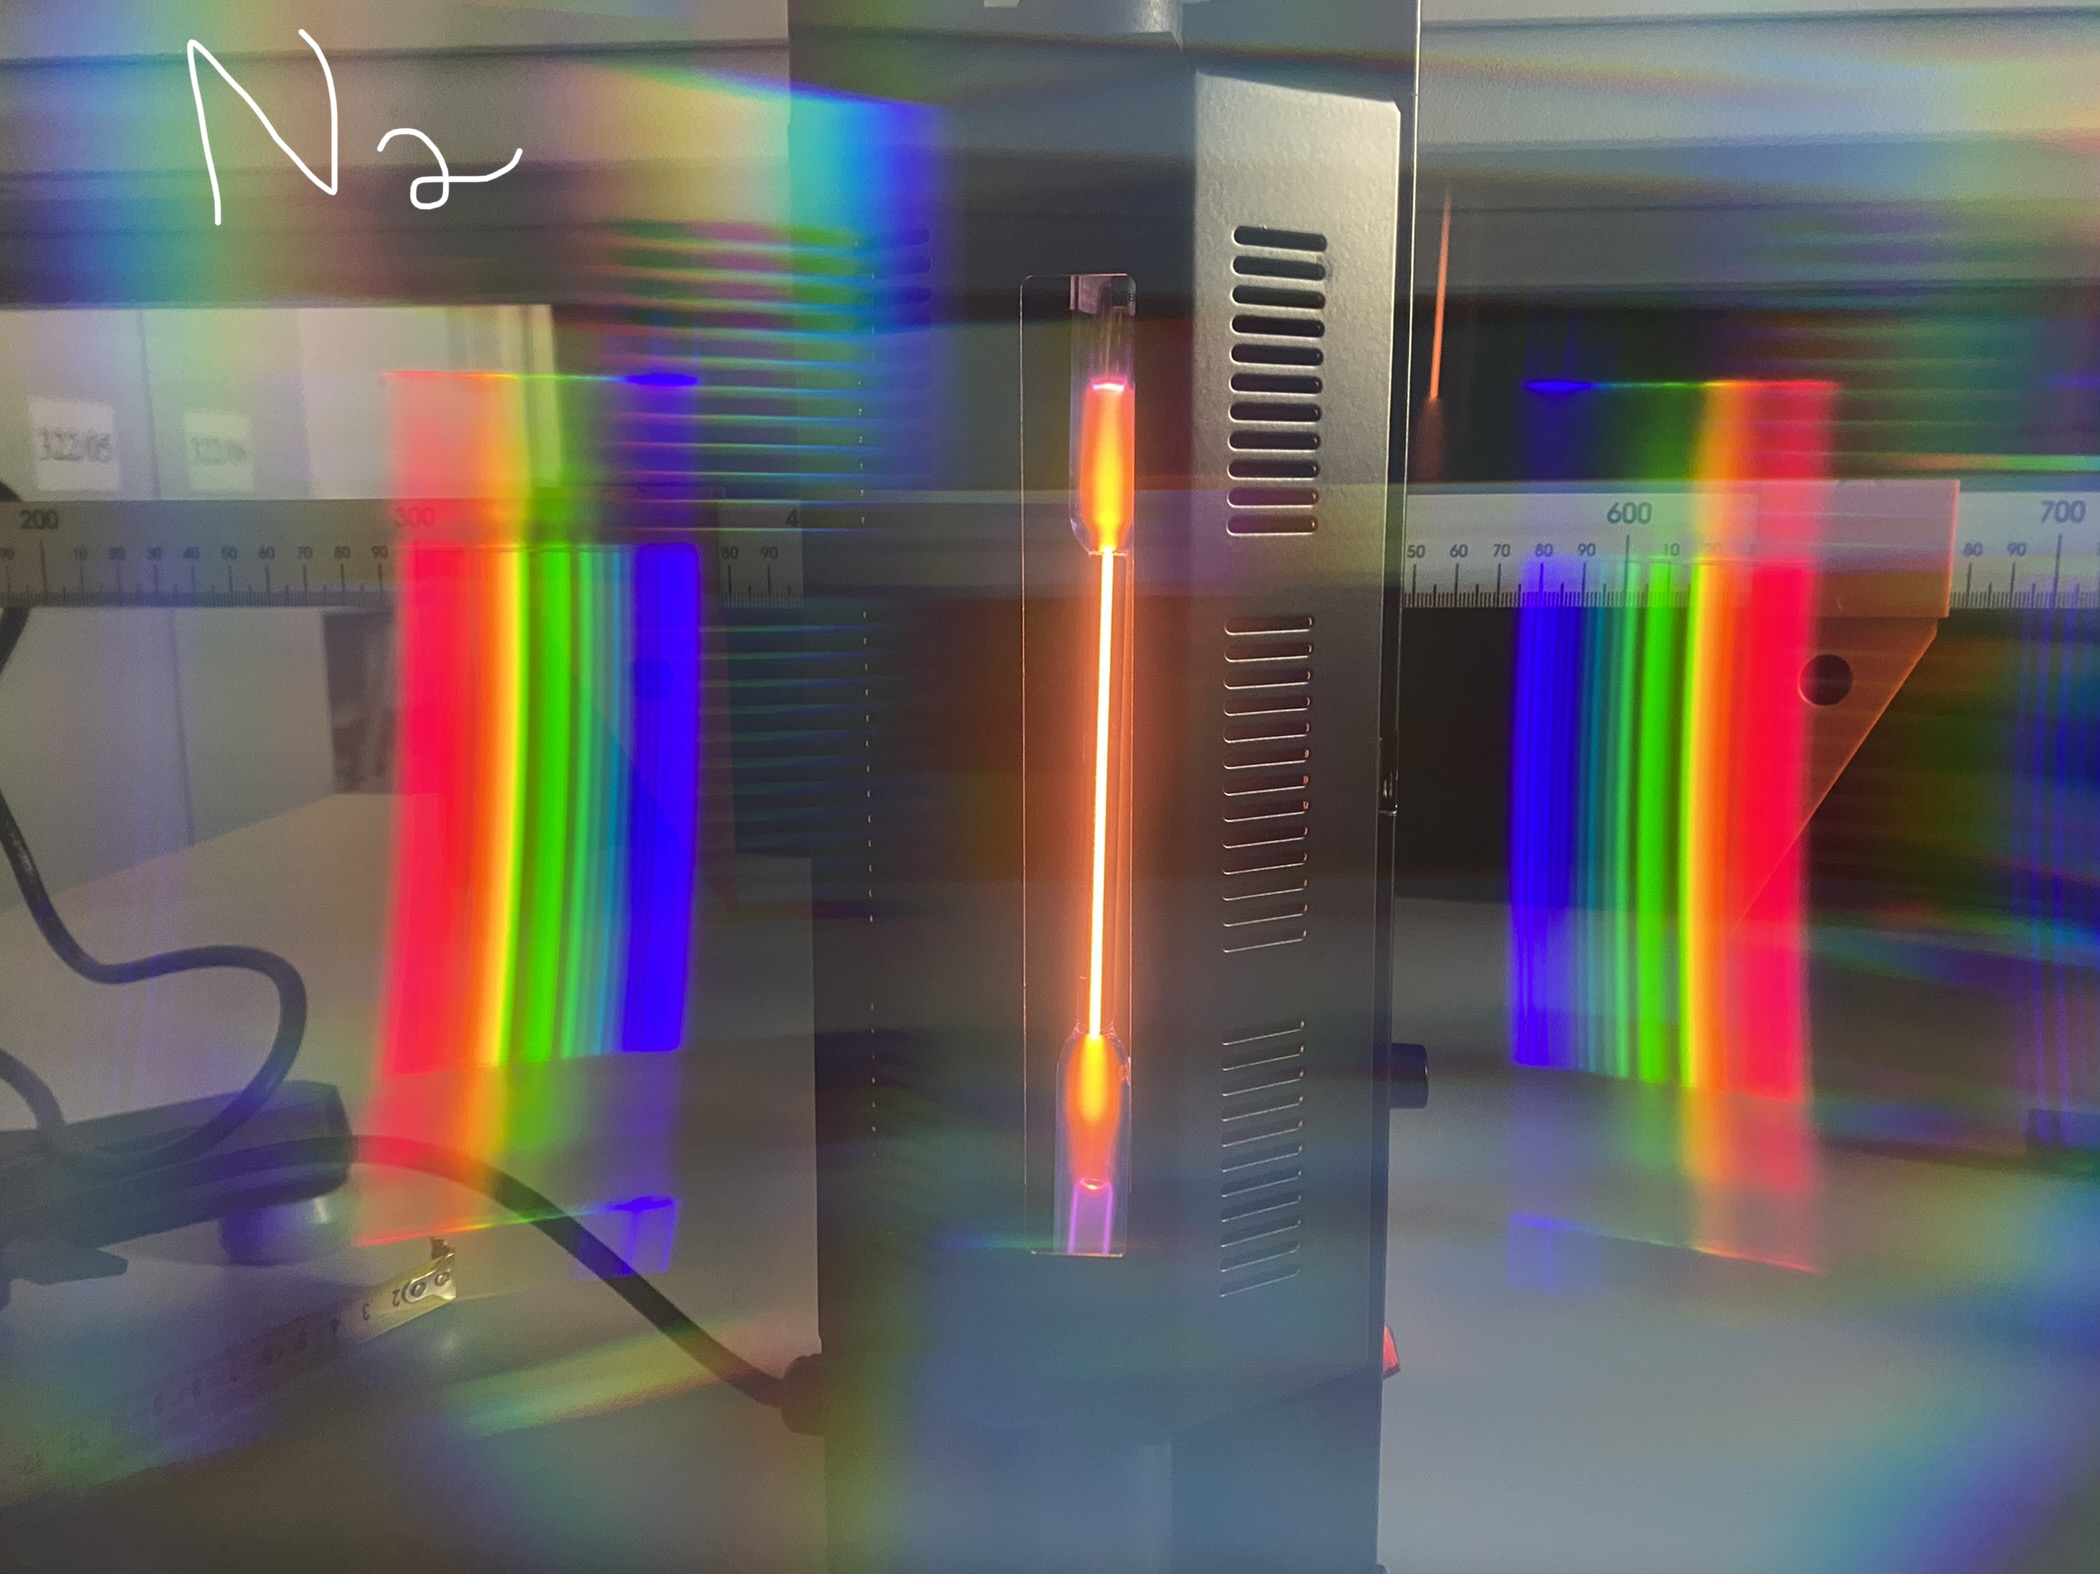
\includegraphics[width=.96\columnwidth]{figures/IMG_5294.jpg}
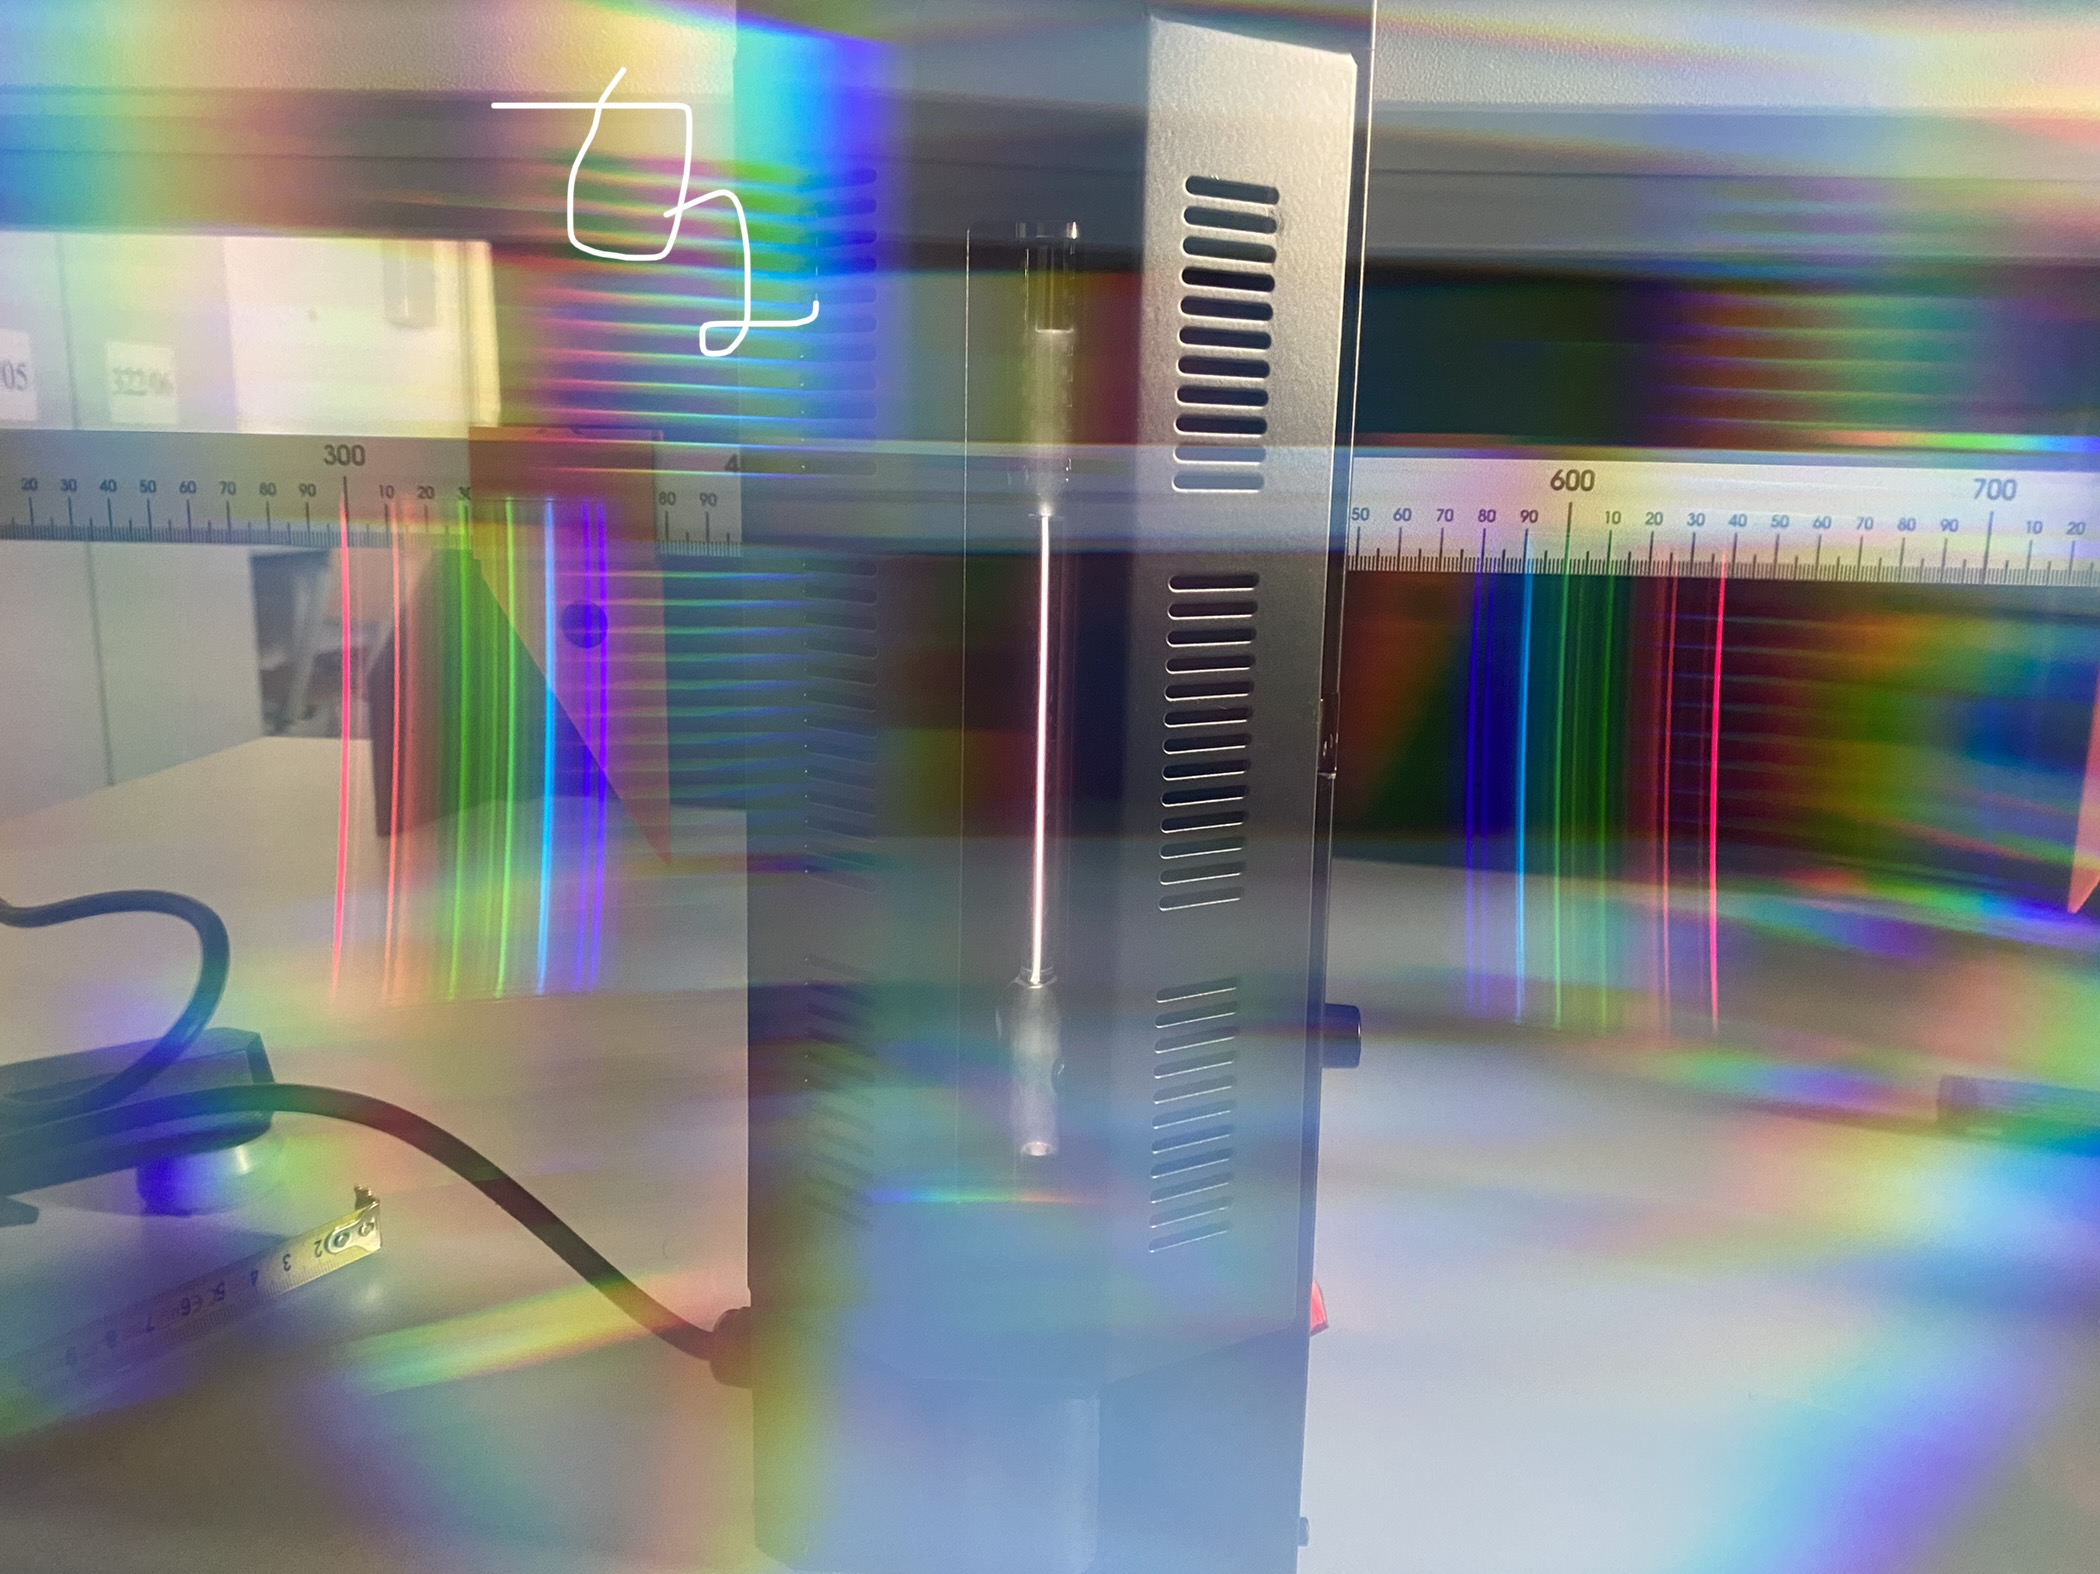
\includegraphics[width=.96\columnwidth]{figures/IMG_5295.jpg}
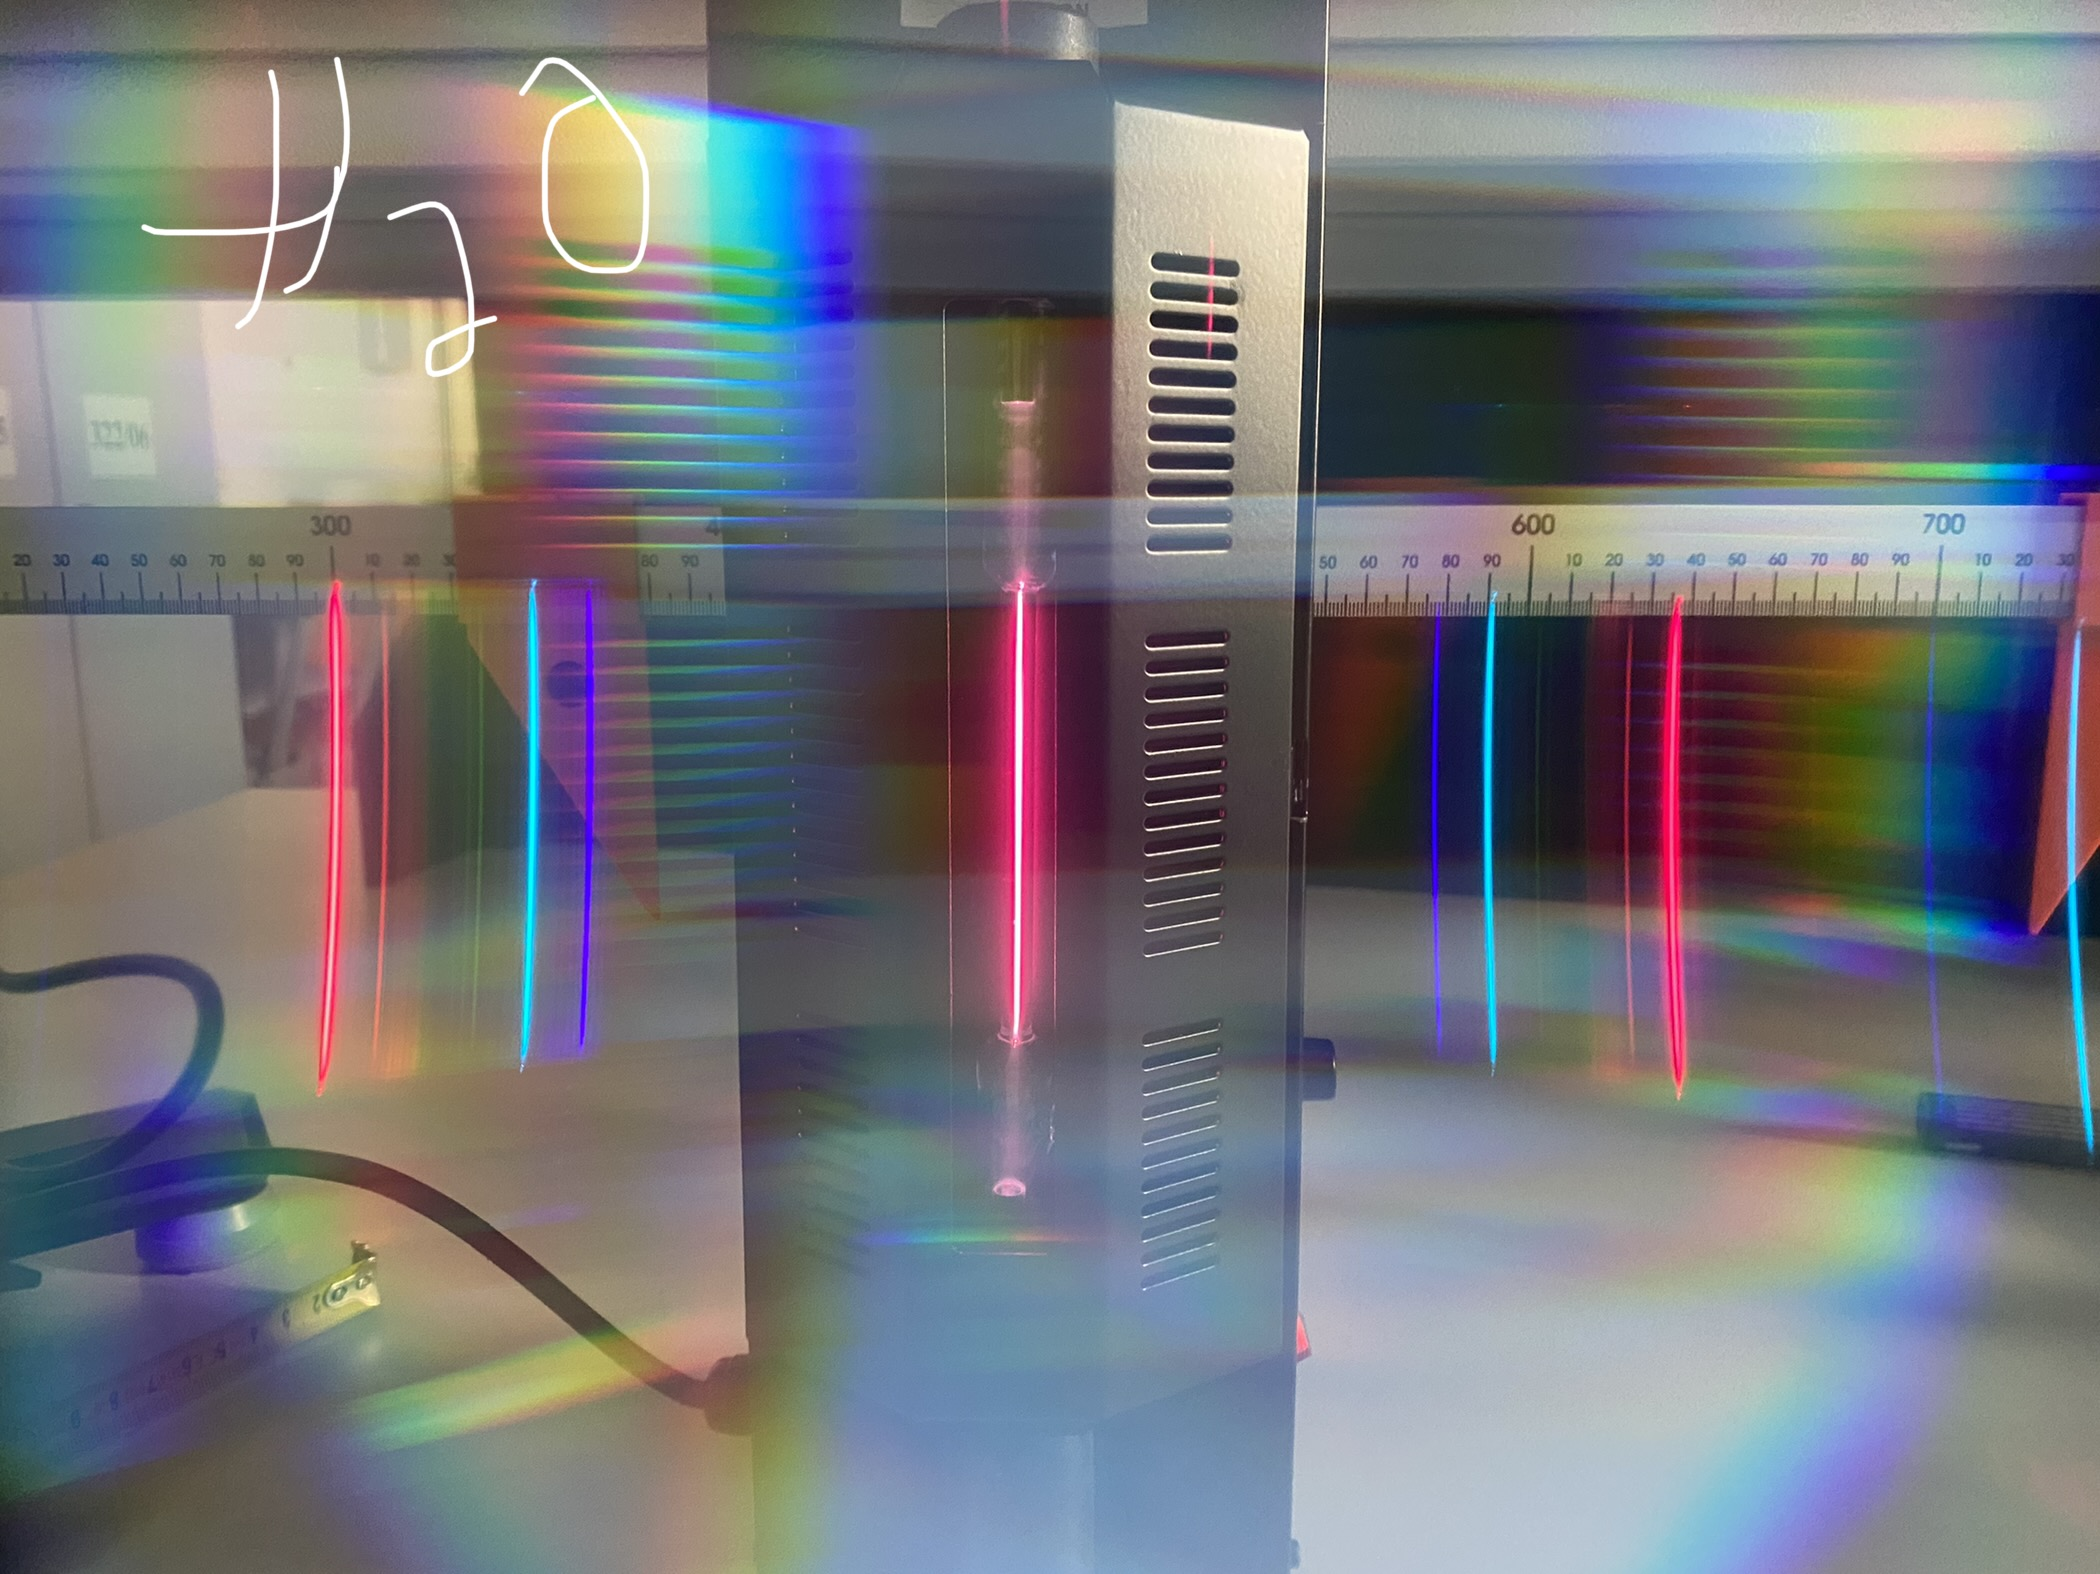
\includegraphics[width=.96\columnwidth]{figures/IMG_5296.jpg}
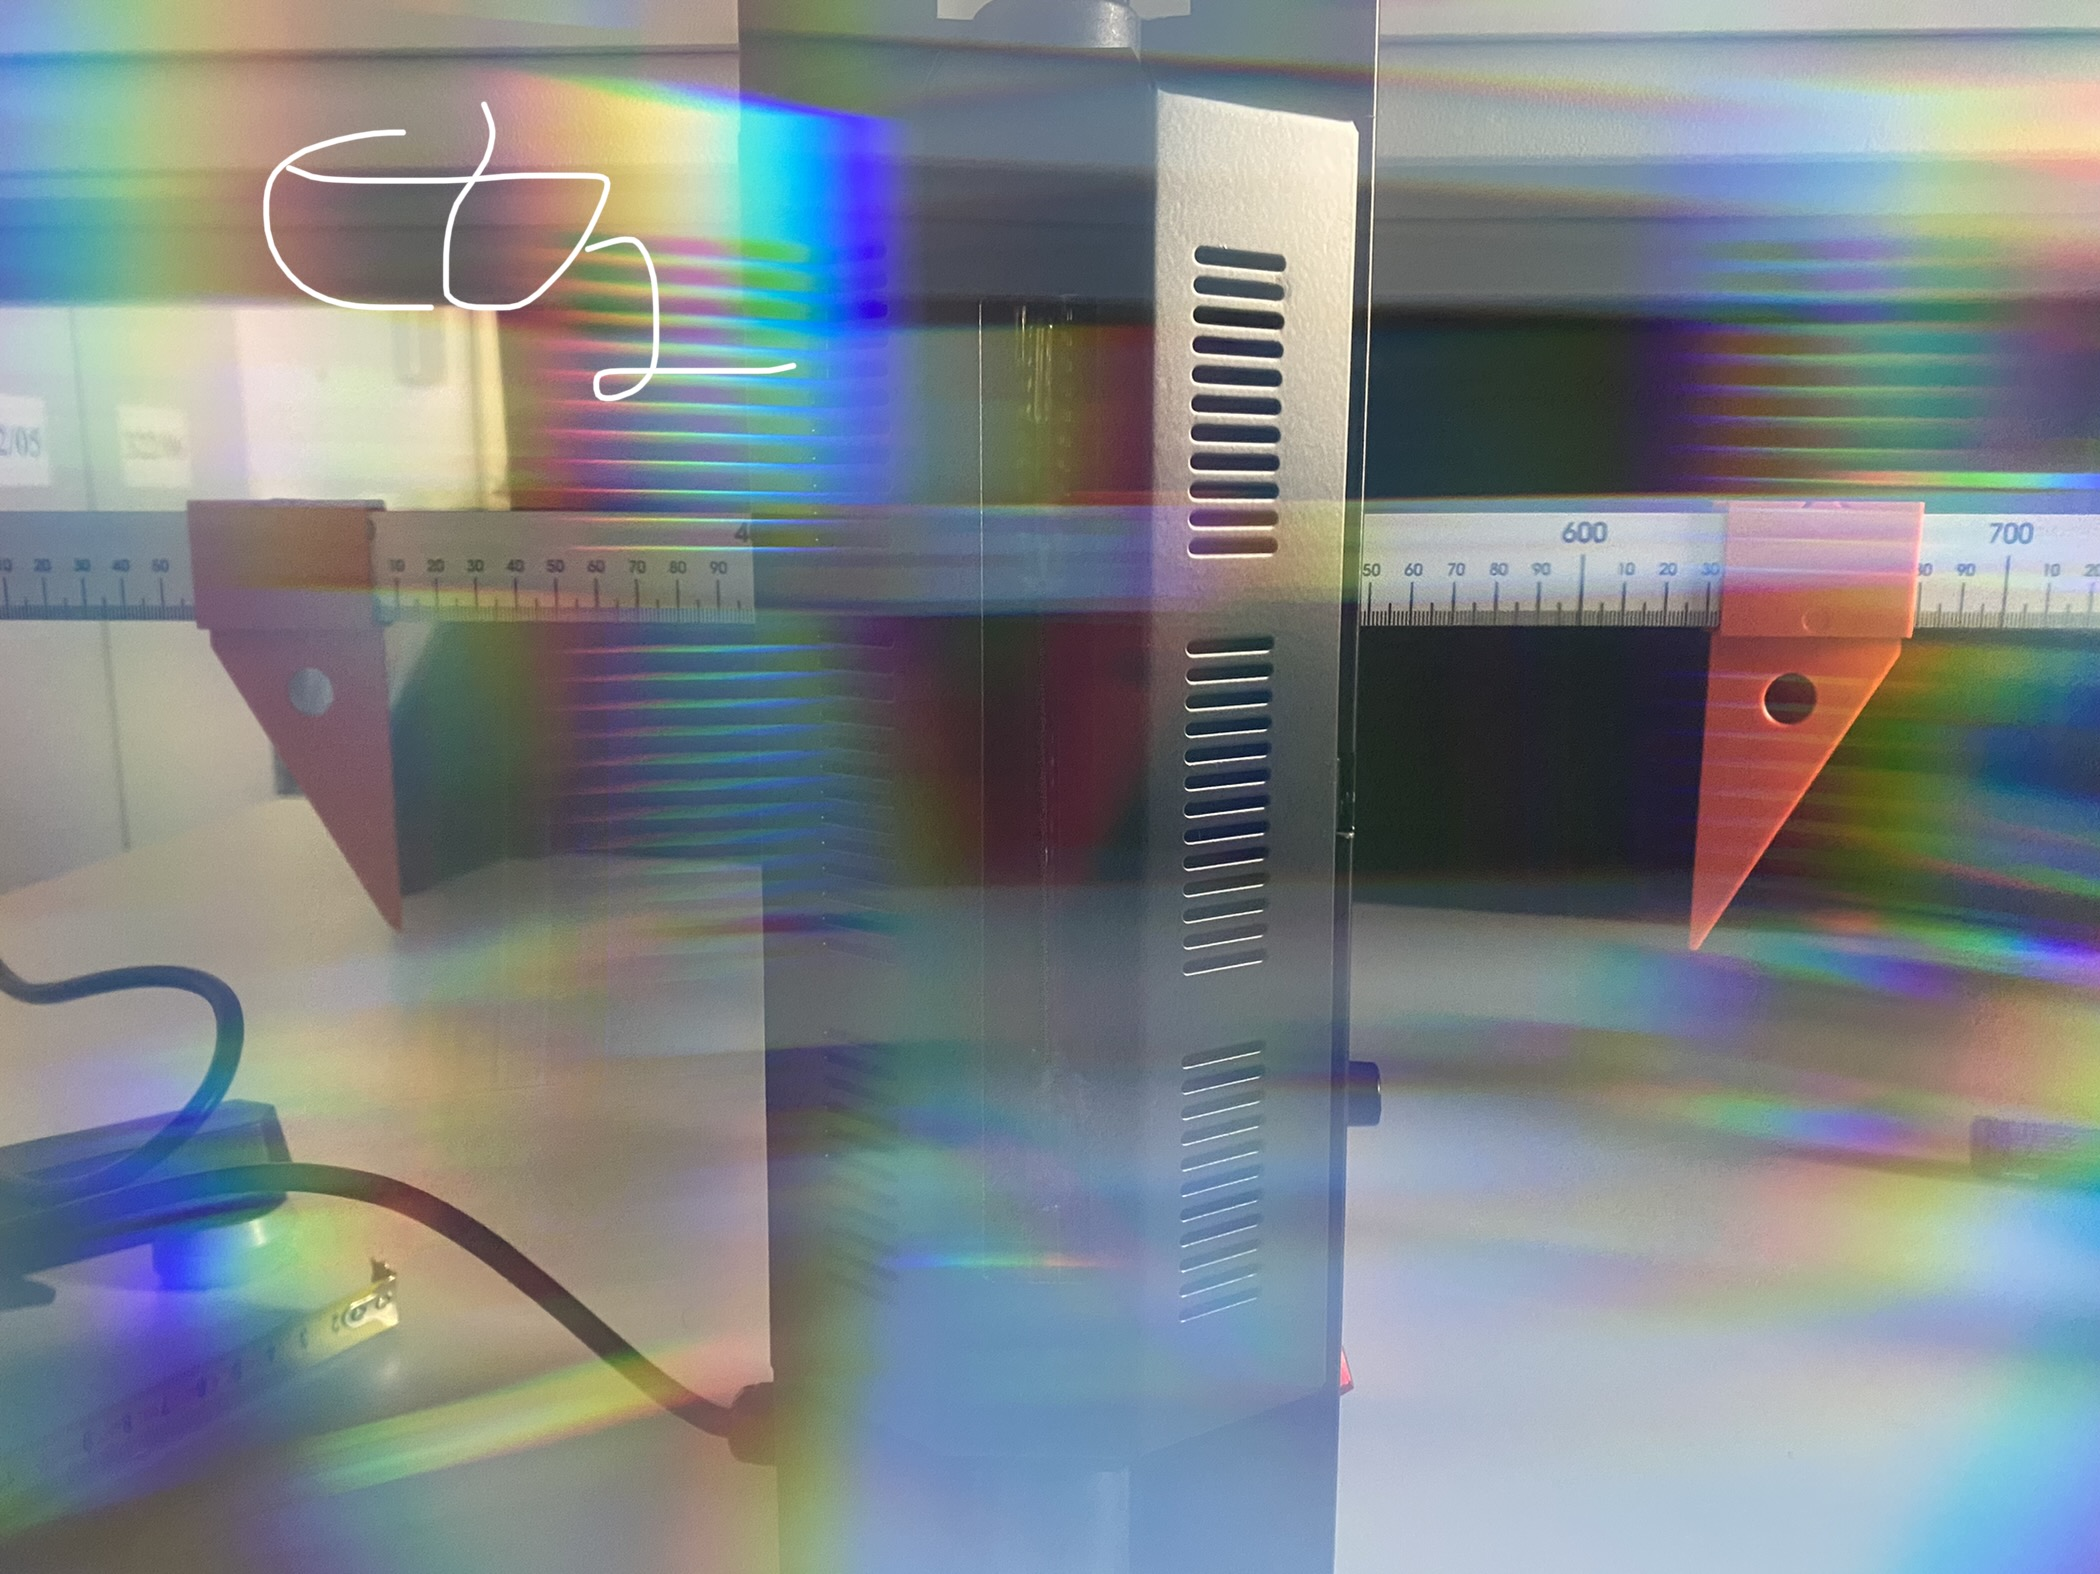
\includegraphics[width=.96\columnwidth]{figures/IMG_5297.jpg}
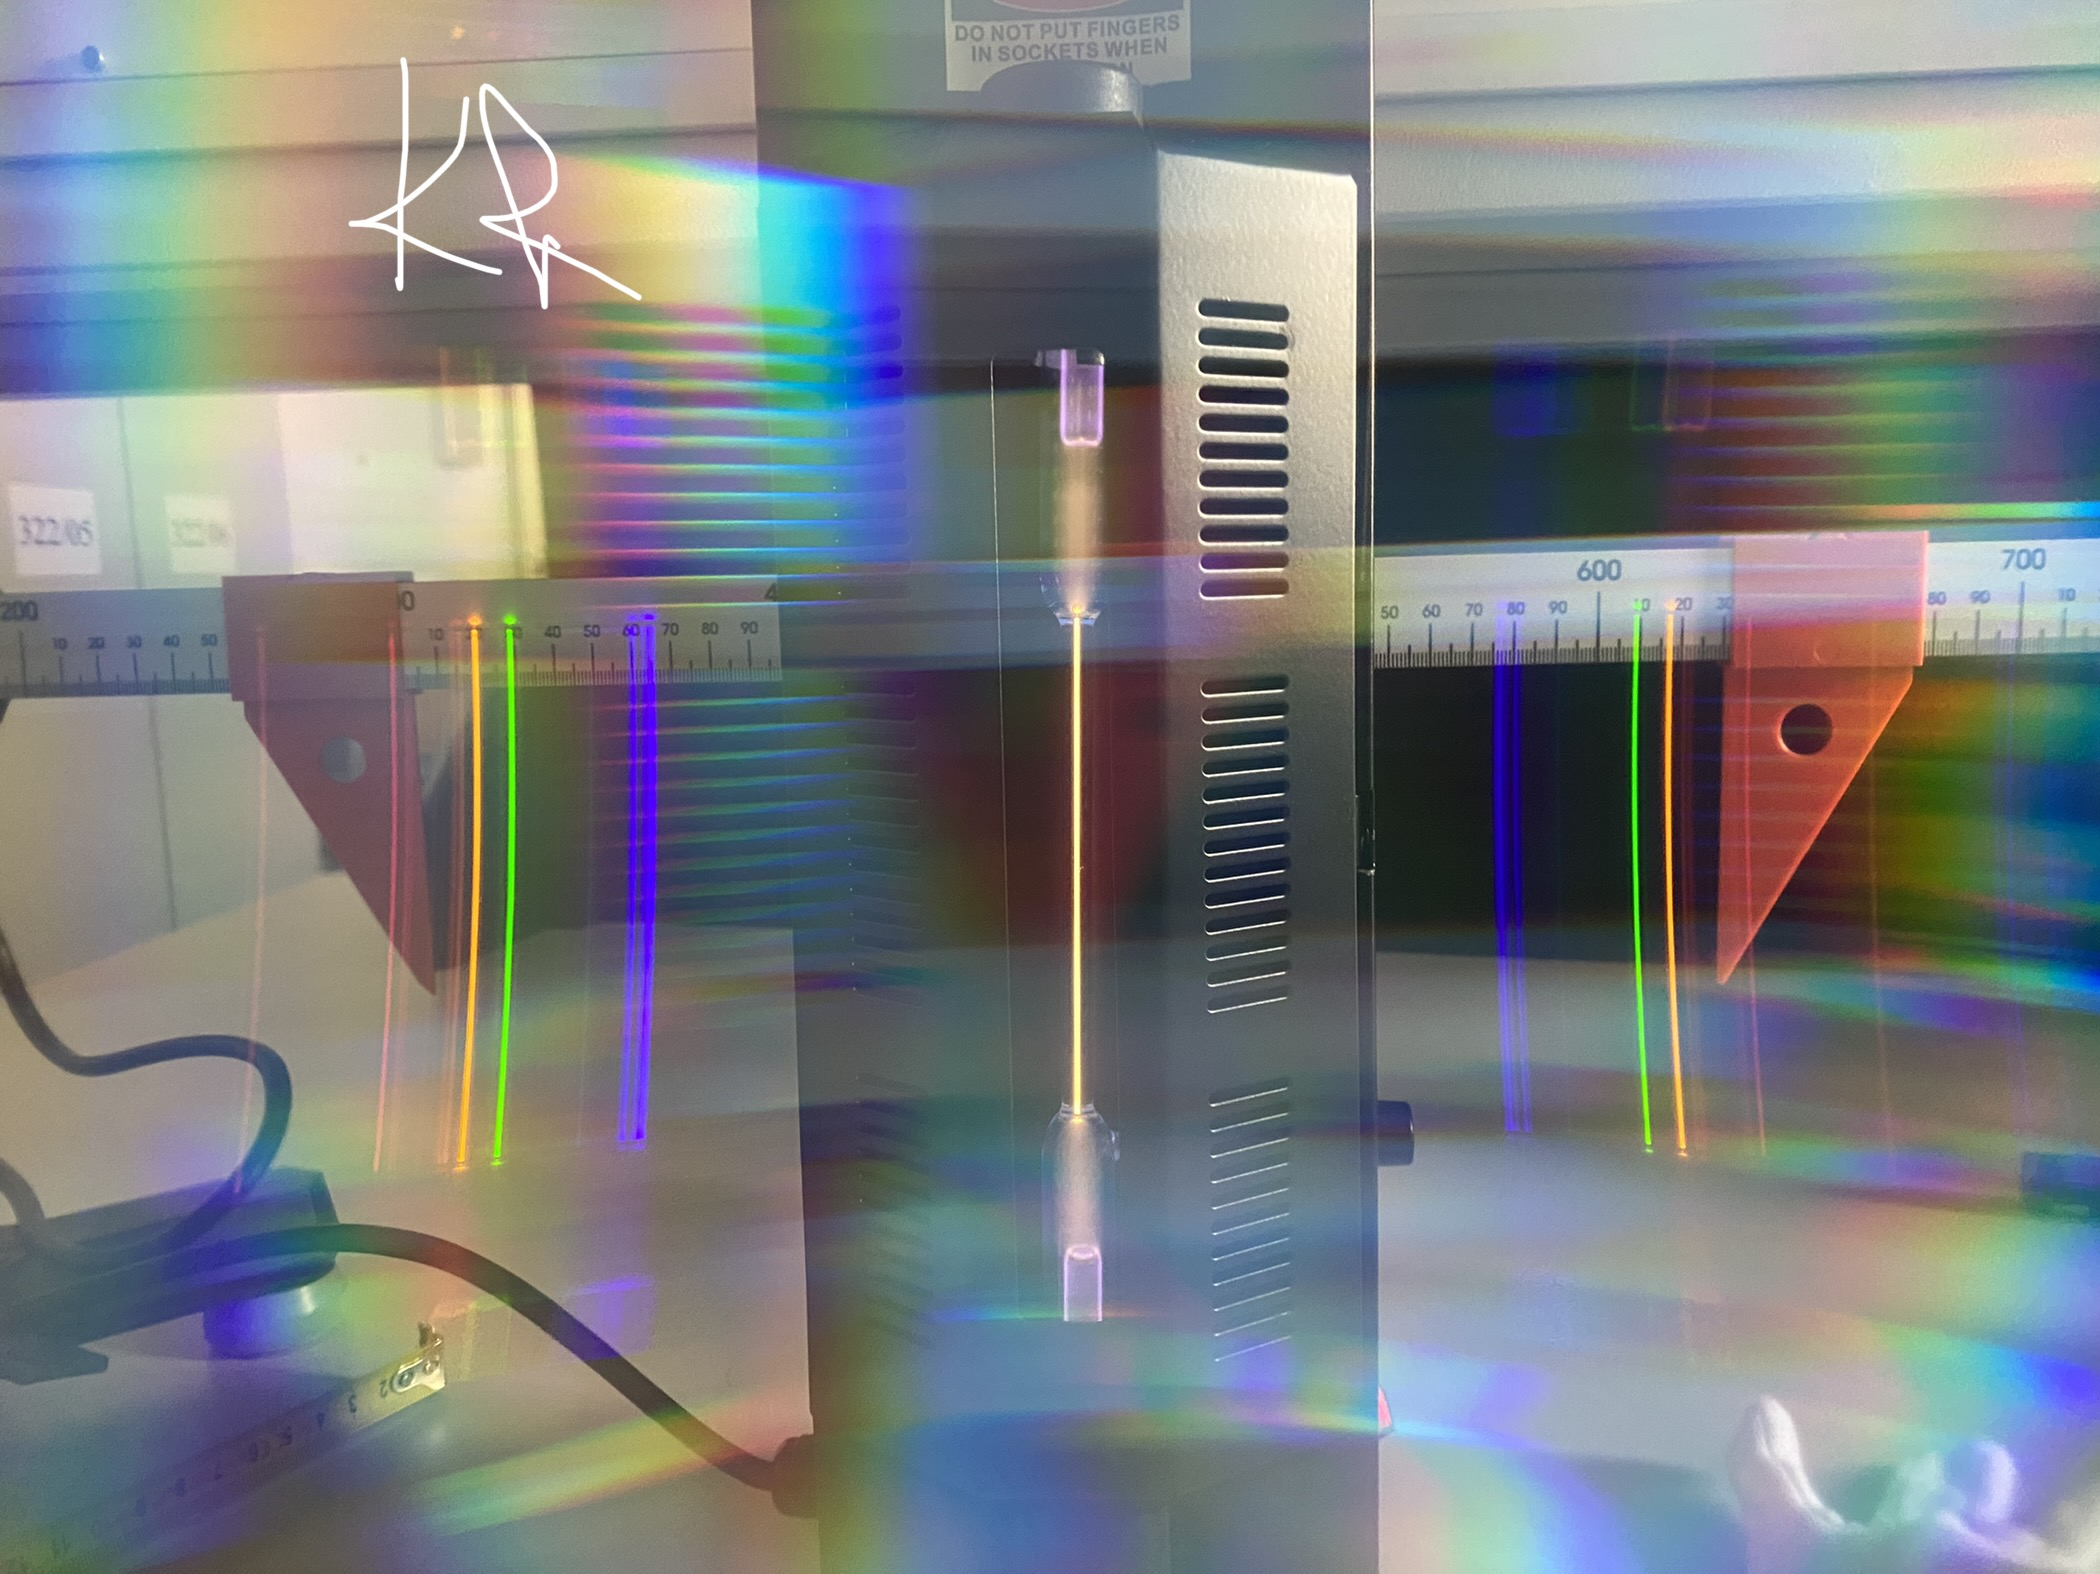
\includegraphics[width=.96\columnwidth]{figures/IMG_5298.jpg}
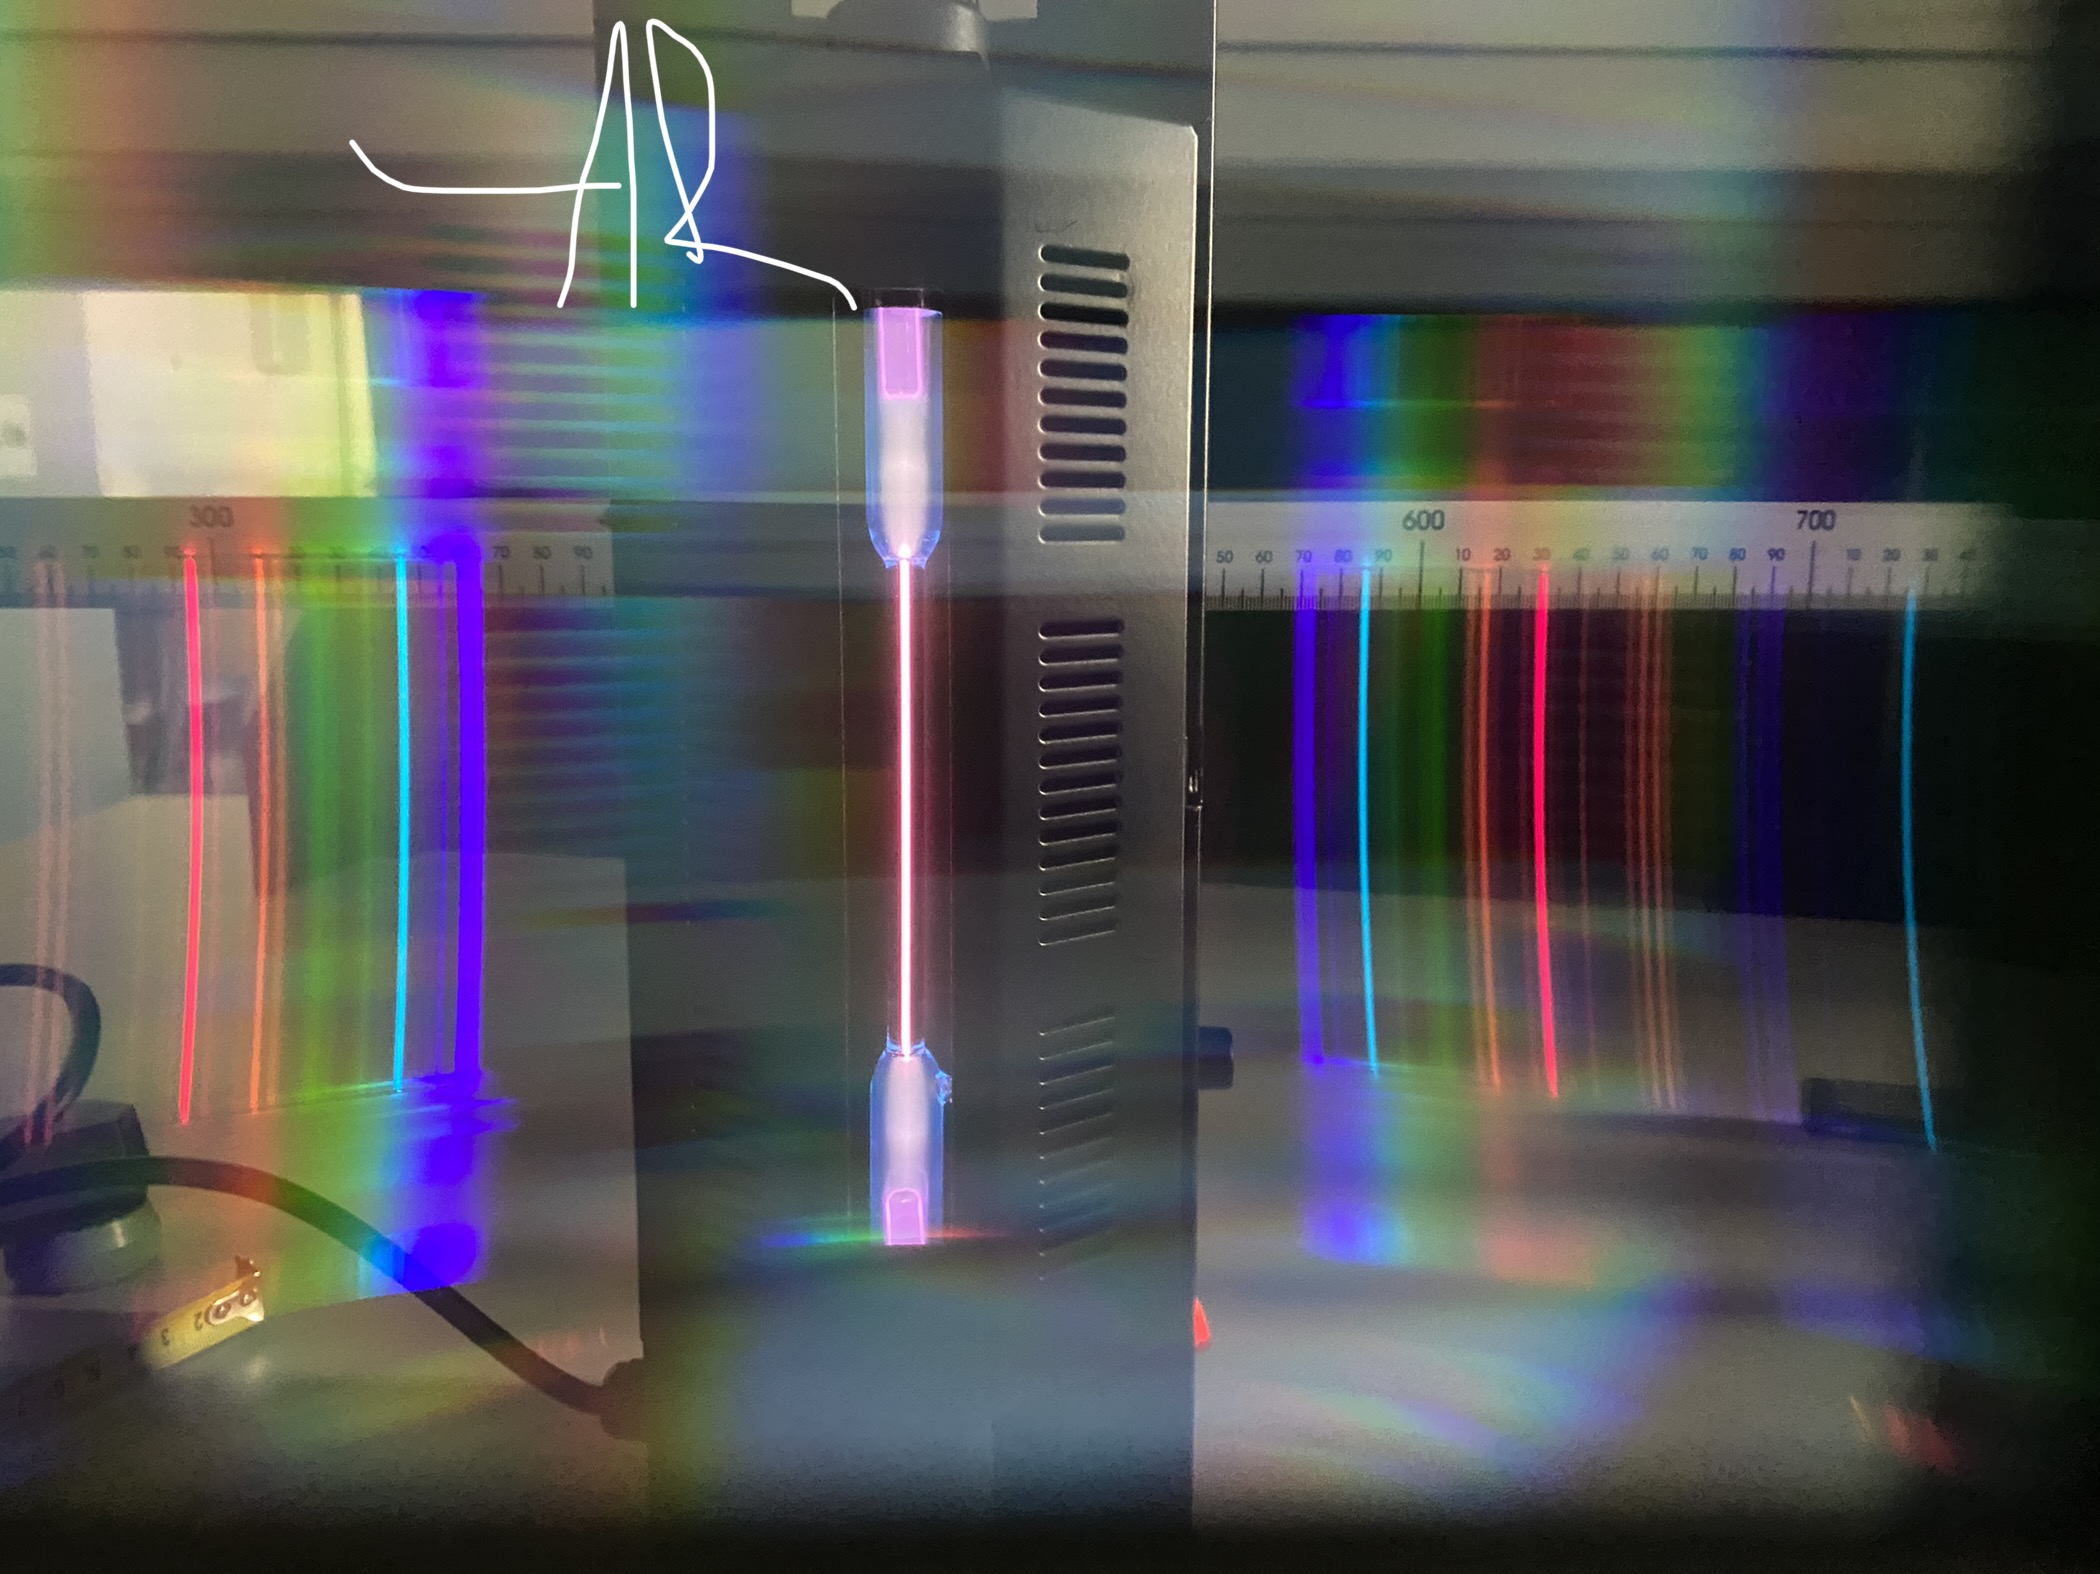
\includegraphics[width=.96\columnwidth]{figures/IMG_5300.jpg}
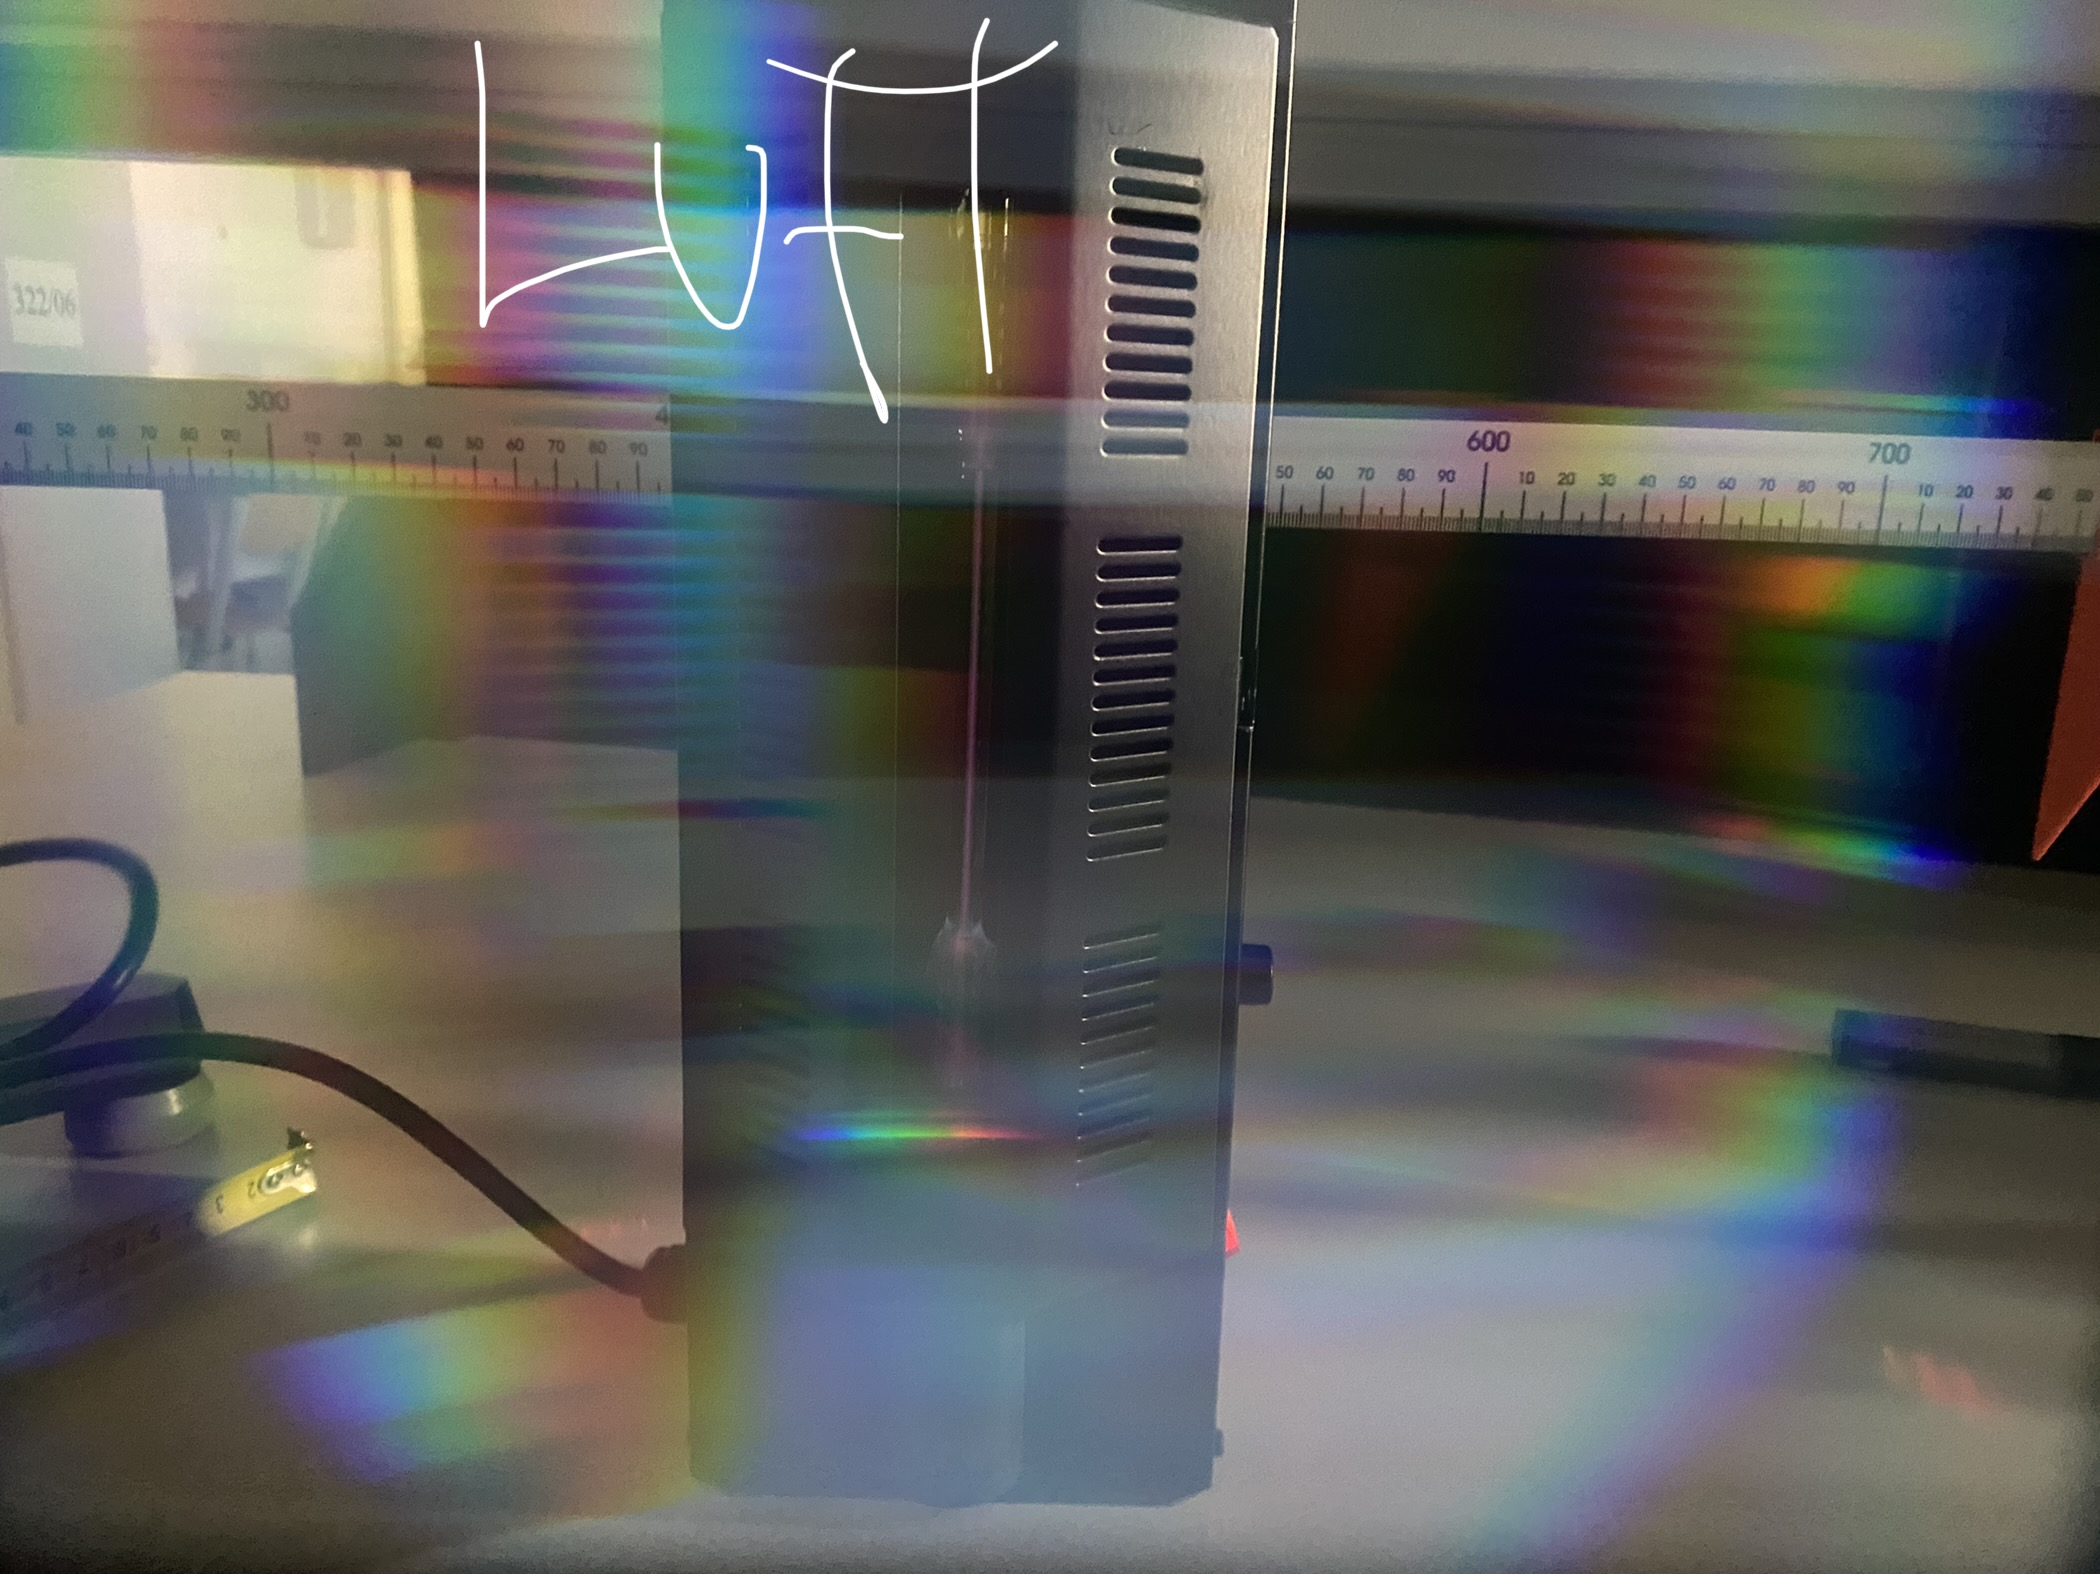
\includegraphics[width=.96\columnwidth]{figures/IMG_5301.jpg}
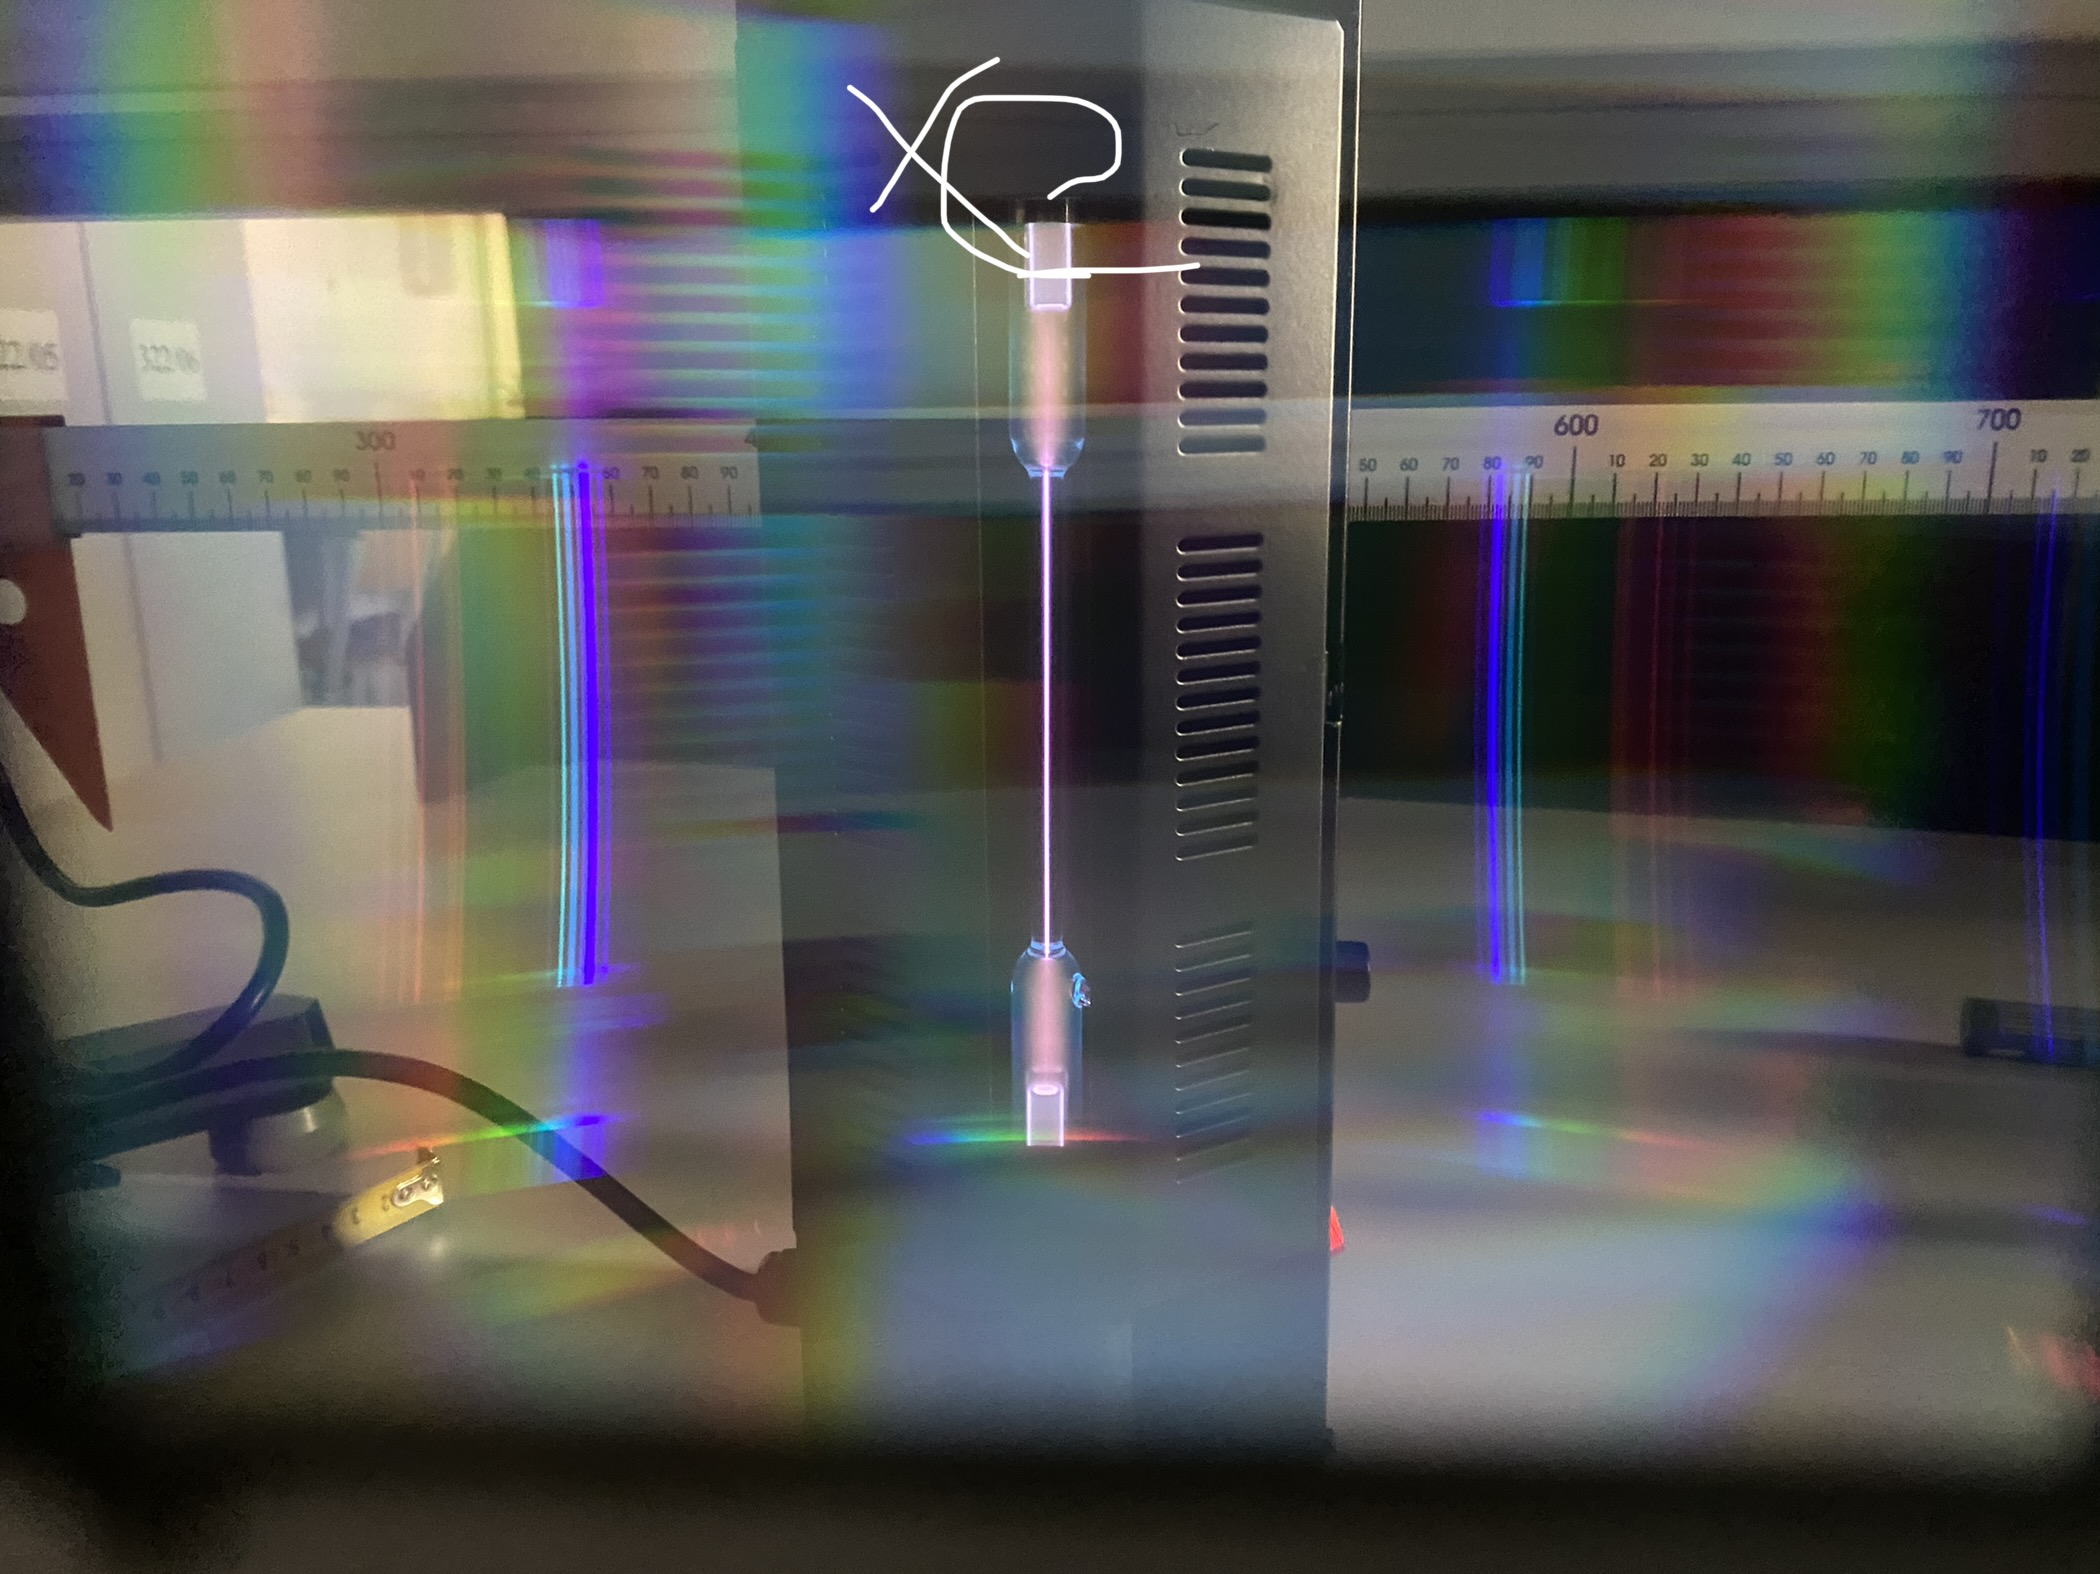
\includegraphics[width=.96\columnwidth]{figures/IMG_5302.jpg}
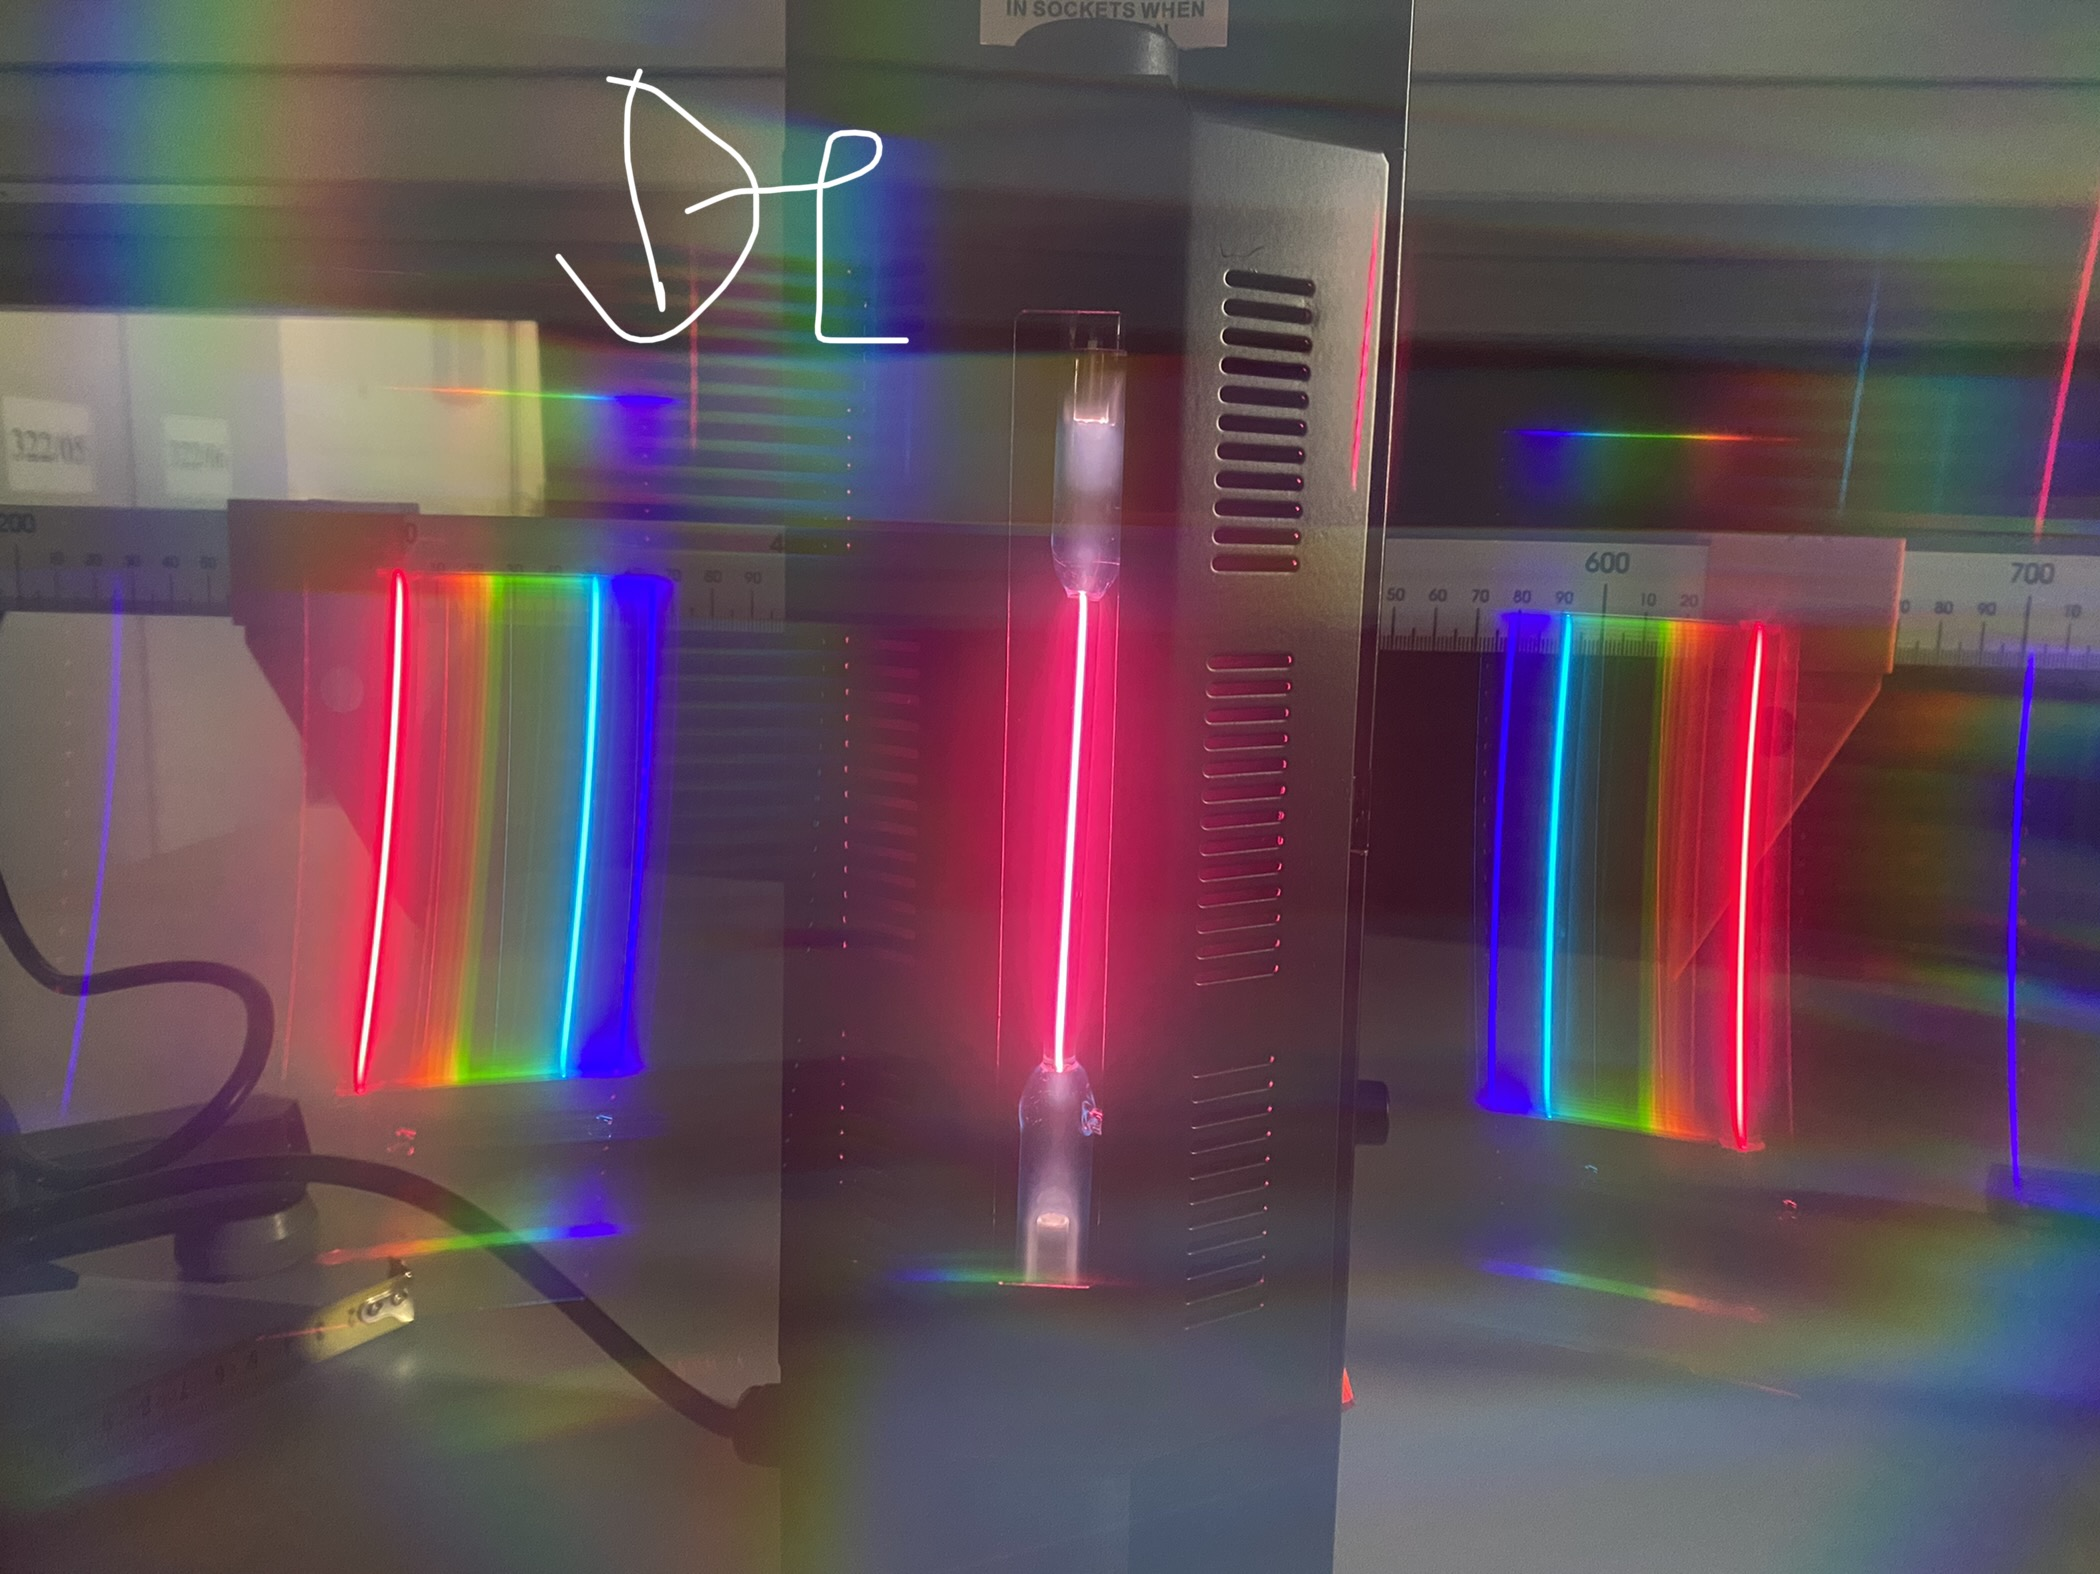
\includegraphics[width=.96\columnwidth]{figures/IMG_5303.jpg}
\section{Anhang - Laborheft}
\includepdf[pages=-,scale=0.9,pagecommand={}]{Laborheft-P3B-SPL.pdf}
       
\end{document}